% THIS IS SIGPROC-SP.TEX - VERSION 3.1
% WORKS WITH V3.2SP OF ACM_PROC_ARTICLE-SP.CLS
% APRIL 2009
%
% It is an example file showing how to use the 'acm_proc_article-sp.cls' V3.2SP
% LaTeX2e document class file for Conference Proceedings submissions.
% ----------------------------------------------------------------------------------------------------------------
% This .tex file (and associated .cls V3.2SP) *DOES NOT* produce:
%       1) The Permission Statement
%       2) The Conference (location) Info information
%       3) The Copyright Line with ACM data
%       4) Page numbering
% ---------------------------------------------------------------------------------------------------------------
% It is an example which *does* use the .bib file (from which the .bbl file
% is produced).
% REMEMBER HOWEVER: After having produced the .bbl file,
% and prior to final submission,
% you need to 'insert'  your .bbl file into your source .tex file so as to provide
% ONE 'self-contained' source file.
%
% Questions regarding SIGS should be sent to
% Adrienne Griscti ---> griscti@acm.org
%
% Questions/suggestions regarding the guidelines, .tex and .cls files, etc. to
% Gerald Murray ---> murray@hq.acm.org
%
% For tracking purposes - this is V3.1SP - APRIL 2009

\documentclass{edm_template}

% Load basic packages
\usepackage{balance}  % to better equalize the last page
\usepackage{graphics} % for EPS, load graphicx instead 
\usepackage[T1]{fontenc}
\usepackage{txfonts}
\usepackage{mathptmx}
\usepackage[pdftex]{hyperref}
\usepackage{color}
\usepackage{booktabs}
\usepackage{textcomp}
\usepackage{booktabs}
\usepackage{comment}
% Some optional stuff you might like/need.
\usepackage{microtype} % Improved Tracking and Kerning
% \usepackage[all]{hypcap}  % Fixes bug in hyperref caption linking
\usepackage{ccicons}  % Cite your images correctly!
% \usepackage[utf8]{inputenc} % for a UTF8 editor only

%\usepackage{algorithm} 
\usepackage[ruled]{algorithm}
\usepackage{algpseudocode}
\usepackage{algorithmicx} 

% If you want to use todo notes, marginpars etc. during creation of your draft document, you
% have to enable the "chi_draft" option for the document class. To do this, change the very first
% line to: "\documentclass[chi_draft]{sigchi}". You can then place todo notes by using the "\todo{...}"
% command. Make sure to disable the draft option again before submitting your final document.
\usepackage{todonotes}

\usepackage{amssymb}
\usepackage{amsmath,scalerel}

\usepackage{graphicx}
\usepackage{epstopdf}
%\usepackage{natbib}
\usepackage{array}
\usepackage{color} 
\newcommand{\hl}[1]{\colorbox{yellow}{#1}}
\usepackage{subcaption}
\usepackage{enumitem}
\usepackage{url}
\usetikzlibrary{arrows.meta,calc,decorations.markings,math,arrows.meta}

\DeclareMathOperator*{\argmax}{arg\,max}
\DeclareMathOperator*{\Bigcdot}{\scalerel*{\cdot}{\bigodot}}

\algnewcommand{\LineComment}[1]{ \State // #1 }

\usepackage{tikz}
\usetikzlibrary{decorations.pathreplacing,calc}
\newcommand{\tikzmark}[1]{\tikz[overlay,remember picture] \node (#1) {};}
\newcommand*{\AddNote}[4]{%
	\begin{tikzpicture}[overlay, remember picture]
	\draw [decoration={brace,amplitude=0.2em},decorate, thick, darkgray]
	($(#3)!(#1.north)!($(#3)-(0,1)$)$) --  
	($(#3)!(#2.south)!($(#3)-(0,1)$)$)
	node [align=center, text width=2.5cm, pos=0.5, anchor=west] {#4};
	\end{tikzpicture}
}%
\usepackage{tabularx}
\usepackage{multirow}


\algdef{SE}[DOWHILE]{Do}{doWhile}{\algorithmicdo}[1]{\algorithmicwhile\ #1}%

\tikzset{
    every picture/.style={
        remember picture,   % Make nodes available to all TikZ pictures
        inner xsep=0pt, % Remove horizontal padding
        inner ysep=1pt, % Set small vertical padding
        baseline,       % Align TikZ pictures at the baseline
        every node/.style={
            anchor=base % Align all nodes at the baseline
        }
    }
}

\begin{document}
	
	\title{Joint Discovery of Skill Prerequisite Graphs \\ and Student Models}
	%\subtitle{[Extended Abstract]
	%\titlenote{A full version of this paper is available as
	%\textit{Author's Guide to Preparing ACM SIG Proceedings Using
	%\LaTeX$2_\epsilon$\ and BibTeX} at
	%\texttt{www.acm.org/eaddress.htm}}}
	%
	% You need the command \numberofauthors to handle the 'placement
	% and alignment' of the authors beneath the title.
	%
	% For aesthetic reasons, we recommend 'three authors at a time'
	% i.e. three 'name/affiliation blocks' be placed beneath the title.
	%
	% NOTE: You are NOT restricted in how many 'rows' of
	% "name/affiliations" may appear. We just ask that you restrict
	% the number of 'columns' to three.
	%
	% Because of the available 'opening page real-estate'
	% we ask you to refrain from putting more than six authors
	% (two rows with three columns) beneath the article title.
	% More than six makes the first-page appear very cluttered indeed.
	%
	% Use the \alignauthor commands to handle the names
	% and affiliations for an 'aesthetic maximum' of six authors.
	% Add names, affiliations, addresses for
	% the seventh etc. author(s) as the argument for the
	% \additionalauthors command.
	% These 'additional authors' will be output/set for you
	% without further effort on your part as the last section in
	% the body of your article BEFORE References or any Appendices.
	
	\numberofauthors{2} %  in this sample file, there are a *total*
	% of EIGHT authors. SIX appear on the 'first-page' (for formatting
	% reasons) and the remaining two appear in the \additionalauthors section.
	%
	\author{%\footnotesize
		\alignauthor{\mbox{\hspace{7em}Yetian Chen$^\star\dagger$,\;\;\; Jos\'{e} P. Gonz\'{a}lez-Brenes$^\dagger$, \;\;\; Jin Tian$^\star$} \\  \hspace{0pt} \\
			\affaddr{$^\star$Computer Science Department}\\
			\affaddr{Iowa State University}\\
			\affaddr{Ames, IA, USA}\\
			\email{\large \{yetianc, jtian\}@iastate.edu}}
		\alignauthor{ \hspace{0pt} \\  \hspace{0pt} \\%Jos\'{e} P. Gonz\'{a}lez-Brenes\\
    		        \affaddr{$^\dagger$Advance Computing and Data Science Lab}\\
			\affaddr{Pearson}\\
			\affaddr{San Diego, CA, USA}\\
			\email{\large jose.gonzalez-brenes@pearson.com}}	
	}
	
\maketitle
\begin{abstract}
Skill prerequisite information is useful for tutoring systems that assess student knowledge or that provide remediation.
These systems often encode prerequisites as graphs designed by subject matter experts in a costly and time-consuming process.
In this paper, we introduce \emph{Combined student Modeling and prerequisite Discovery} (COMMAND), 
a novel algorithm for jointly inferring a prerequisite graph and a student model from data.
Learning a COMMAND model requires student performance data and a mapping of items to skills ($Q$-matrix).
COMMAND learns the skill prerequisite relations as a Bayesian network (an 
encoding of the probabilistic dependence among the skills)
via a two-stage learning process. 
In the first stage, it uses an algorithm called Structural Expectation Maximization to select a class of equivalent Bayesian networks; % based on distribution fitting of student data;
in the second stage, it uses  curriculum information to select a single Bayesian network.
Our experiments on simulations and real student data suggest that COMMAND is better than prior methods in the literature.

% the pipeline estimates the causal structure and the probabilistic dependence among the skills 
%via a two-stage learning process. 
%In the first stage, the Structural Expectation Maximization (Structural EM) algorithm is used to select a class of Bayesian networks based on distribution fitting of student data;
%in the second stage, a single Bayesian network structure is determined by enforcing a constraint on the estimated conditional probability tables.
%We validate the proposed pipeline using simulations and by post-hoc analysis of student data.
%We show the discovered prerequisite structures can improve the student model in predicting student performance. 
\end{abstract}

%% A category with the (minimum) three required fields
%\category{H.4}{Information Systems Applications}{Miscellaneous}
%%A category including the fourth, optional field follows...
%\category{D.2.8}{Software Engineering}{Metrics}[complexity measures, performance measures]
%
%\terms{Theory}

\keywords{Prerequisite discovery, Bayesian network, student modeling} % NOT required for Proceedings

\section{Introduction}
\label{sec:introduction}
Course \textit{curricula} are usually organized in a meaningful sequence  that evolves from relatively simple lessons to more complex ones. 
%Students learn much better when the skills are not randomly introduced 
%but organized in a meaningful order which starts from relatively simple concepts and gradually introduces more complex ones. 
Among these lessons, some are required to be mastered by the student  before the subsequent ones can be learned.
For instance, students have to know how to do addition before they learn to do multiplication.
We refer to \textit{prerequisite structure} as the relationships among skills that place strict constraints on the order in which  skills can be acquired. 

Prerequisite structures are crucial for designing intelligent tutoring systems that assess student knowledge or that offer remediation interventions to students.
Building such systems require prerequisite information that is often hand-engineered by subject matter experts in a costly and time-consuming process. 
Moreover, the prerequisite structures specified by the experts are seldom tested and might be unreliable in the sense that experts may have ``blind spots".

%Nowadays, large volume of educational data has been cumulated through the digital tutoring systems.  
%Thus, learning prerequisite structures from educational data has drawn substantial interest from both education and data mining communities \cite{desmarais2006learned,vuong2010method, brunskill2010estimating,scheines2014discovering,chen2015discovering,piech2015deep}.
%However, inferring the prerequisite relationships between skills is still challenging since a student's knowledge of a skill is an unobserved latent variable in the data.

Recent interest in computer assisted education promises large amounts of data from students solving \textit{items}--- questions, problems, parts of questions.
Performance data --what items a learner answers correctly-- can be used to create \textit{student models}. % that predict future performance.
These models represent an estimate of skill proficiency  at a given point in time~\cite{vanlehn1988student}.
For example, a student model can represent that Alice has  already mastered integer addition, but Bob has not.
Student models are often used to personalize instruction in tutoring systems or to predict future student performance.
In this paper, we introduce \emph{Combined student Modeling and prerequisite Discovery} (COMMAND), 
a novel algorithm for simultaneously discovering prerequisite structure of skills and a student model from student performance data.

%In education, remedial interventions attempt to eliminate the specific effect of lacking a competency.
%Traditional and mastery-based educational strategies~\cite{bloom1968learning} often rely on remedial interventions when a learner is having a difficulty in the curriculum.
%Teachers often use their experience, knowledge and common sense to justify if a student may need remedial assistance.
%With the growing popularity of Intelligent Tutoring Systems, computers are starting  to have capabilities to detect when a student is in need of remediation.
%The process of designing when a computer should offer remediation to a student typically starts by subject matter experts writing rules that are then engineered into the system.
%These rules are difficult and time consuming to build.


%In this paper we introduce the \textit{Remedial Intervention Detector} (REMIND) algorithm.
%REMIND is a novel pipeline that uses data--and optionally domain knowledge-- to infer when a student may lack the  necessary  knowledge to solve the current lesson.
%We believe the capability of combining data with subject matter expertise is a promising approach.


%\section{Remedial Intervention Detector (REMIND) }
%In many instructional settings, students are graded by their performance on instruments such as exams or homework assignments. 
%Usually, these instruments are made of items--questions, problems, parts of questions-- which are graded individually.
%Modern applications of statistics in education often rely on a mapping of items to skills (often called a $Q$-matrix) to analyze data collected from students answering items.
%The item to skill mapping is often designed by subject matter experts, but automatic approaches exist~\cite{jp_aistats_2015}.
%
%REMIND is a pipeline that uses data from students answering items to discover when a student  is lacking background knowledge and could benefit from remediation.
%For this, REMIND first discovers prerequisite structures  among the skills in the data.
%In the context of this paper, we define the prerequisite structure as the strict constraints on the order in which these skills can be acquired.
%REMIND then uses student modeling techniques to infer if a student has mastered the skill and its prerequisites.
%The rationale is  that a student should receive a remedial intervention if she is likely to lack a prerequisite.%, an intervention for tutoring remedial content should be offered to the student.
%In \S~\ref{sec:learning_remind} we describe how to learn a REMIND  model from data;
%and in \S~\ref{sec:using_remind} we explain how to use it to offer remedial interventions.


\section{Relation to Prior Work}
\label{sec:previous_work}

Prior work has investigated how to discover %the discovery of prerequisite structures from data.
%Many of these approaches discover 
 prerequisites among items without considering their mapping into skills~\cite{desmarais2006learned,vuong2010method}. %,piech2015deep}. I don't think this paper is relevant
Item-to-skill mappings (also called $Q$-matrices) are desirable because they allow more interpretable diagnostic information.
%That is, the prerequisites do not use skill mappings, 
%and only find dependencies between items
%These include the Partial Order Knowledge Structures (POKS) algorithm \cite{desmarais2006learned, pavlik2008using} to learn the item-item relationships
%and an approach to determine the dependency structure of units in a curriculum with the student performance observed at the unit level \cite{vuong2011method}.
%To learn the relationships among skills from data where a student's knowledge of a skill is latent, 
%To account for latent skills, a mapping of items to skills (often called a $Q$-matrix) is used.
%In this setting, students are tested on items-questions, problems, parts of questions- 
%each of which requires one or multiple background skills.
%To estimate the relationship between two background skills, 
Because of this, follow-up work~\cite{brunskill2010estimating,chen2015discovering}  has studied whether a pair of skills have a prerequisite relationship or not.
%They do so by comparing data of a pair of skills using  two different models.
%They do so by comparing two models that represent different relationships between two skills.
For this,  we can measure if a model that assumes a dependency between the two skills explain the data better than a model that assumes independence. %if there is a prerequisite relationship between a pair of skills or not.
This comparison can be done with data likelihood~\cite{brunskill2010estimating} or association rule mining~\cite{chen2015discovering}.
Although  promising, prior methods have   limitations that we address:
%\vspace{-5mm}
\begin{enumerate}%[itemsep=0mm]
\item We estimate the global prerequisite structure, not just the pairwise relationships. % between skills and do not optimize the entire prerequisite structure.
For example, suppose we want to discover the prerequisites of three skills for English learning ($S_1$:syntax, $S_2$:cohesion and $S_3$:lexical rules).
If we use prior methods we discover that the three skills are related among each other.
%but we are unable to know if syntax requires directly both cohesion and lexical rules, or if the effect is through an indirect pre
However, pairwise relations are unable to tell if the relationship is due to indirect effects  (e.g, $S_3 \rightarrow S_2 \rightarrow S_1$), or due to a skill with two prerequisites (e.g, 
$S_3$\tikz \node(a) {\vphantom{g}};$\rightarrow S_2 \rightarrow$\tikz \node(b) {\vphantom{g}};$S_1$%
 \tikz [overlay] \draw [->]  (a.south) to [bend right=18]  (b.south);).
 
\item It is unclear how to use the output of these prerequisite structures for student modeling. For example,  to make predictions of future student performance.
\item Prior work does  not provide a quantitative evaluation using real student data. Overall, prior work has used real student data for examples, but without any quantitative evaluation methodology that can help compare different techniques.
\end{enumerate}
%Prior work has evaluated their methods using simulated data, and limited student data for examples.
%\vspace{-5mm}
%Moreover, these approaches require many preconditions. For example, Brunskill's method assumes domain parameters called \emph{guess probability} and \emph{slip probability} are provided for each pair of item and skill.
%Chen et al's approach requires manually specified thresholds to determine the existence of a prerequisite relationship.
%The determination of these thresholds requires experts' intervention. 

A statistical formalism called Bayesian network has been useful to model prerequisite structures~\cite{mislevy1999bayes}. 
%\hl{I think Bob Mislevy had one of the first seminal papers of using BNs in education}
Bayesian networks allows  modeling the full structure of skills (beyond pairwise relationships) and can encode conditional independence  between the skills.
%Modeling the full structure is appealing to enable more accurate modeling.
Unfortunately, prior work with Bayesian networks requires a domain expert to design the prerequisite structures~\cite{kaser2014beyond},
and automatic techniques have not been demonstrated with real student data~\cite{scheines2014discovering}.
We now describe the COMMAND algorithm that discovers a Bayesian network that encodes the prerequisite structure of skills.
%A secondary contribution of COMMAND is that  that it \hl{may} allow for minimal domain knowledge to discriminate between statistically equivalent  networks.

%By modeling prerequisite relations as a Bayesian network, Scheines et al. converted the problem of prerequisite structure discovery to a Bayesian network structural learning problem, and proposed an algorithm to find Bayesian network structures that fit the data \cite{scheines2014discovering}.
%However, the output from their algorithm is a class of Bayesian networks, which are equivalent in representing a probability distribution.
%These \emph{equivalent} Bayesian networks have the same skeleton but differ in the orientation of some edges, thus represent very different prerequisite structures.
%Scheines and his colleagues did not offer any solution to discriminate between these Bayesian networks.
%Further, they validated their algorithm only on synthetic data

\begin{comment}
In this paper, we propose the \emph{Combined student Modelling and prerequisite Discovery} (COMMAND) pipeline 
to infer the prerequisite structures of skills and a student model from data. 
The pipeline also uses the promising Bayesian network model to represent the prerequisite relationships.
The pipeline first uses a popular Bayesian network structure learning algorithm, 
called Structural EM to select a class of Bayesian network models based on the distribution fitting of the data.
It then uses the domain knowledge that it is unlikely for a student to master a skill before mastering its prerequisite skills to select one Bayesian network, 
which gives a unique prerequisite structure.
Different from \cite{scheines2014discovering}, Structural EM converts the Bayesian network learning to an optimization problem.
It is more scalable and can be applied to data that contain missing values.
Further, the approach in \cite{scheines2014discovering} only outputs the topology of the Bayesian network, while 
Structural EM outputs both the structure and the probability distribution (a set of conditional probabilities), which is very useful for student modeling.
We demonstrate the robustness of our proposed approach on noisy data that contains unaccounted latent variables or missing values.
Finally, we show the discovered prerequisite models are useful for student modeling.
%\hl{ Please consider adding a table \url{https://docs.google.com/document/d/1BTNJSc67-vAUkSsDBp8b1OyvClQULx42b6PyQXQ3it4/edit}}
\end{comment}





\section{The COMMAND Algorithm}
\label{sec:pre_pipeline}
COMMAND learns the prerequisite structure of the skills from data with a statistical model called Bayesian network \cite{pearl1988probabilistic,spirtes2001causation}.
Bayesian networks are one type of probabilistic graphical models because they can be represented visually and algebraically as a collection of nodes and edges.
A tutorial description of Bayesian networks in education can be found elsewhere \cite{mislevy1999bayes}, 
but for now we say that they are often described with two components: 
the  nodes represent the random variables, which we describe using \textit{conditional probability tables} (CPTs),
and the set of edges that form a \textit{directed acyclic graph} (DAG) represent the conditional dependencies between the variables.
Bayesian networks are a flexible tool that can be used to model an entire curriculum.

 

Figure~\ref{fig:smexample} illustrates an example of a prerequisite structure modeled with a Bayesian network.
Here, we relate four test items with the skills of addition and multiplication.
Addition is a prerequisite of multiplication thus there is an arrow from addition to multiplication.
Modeling prerequisites as edges in a Bayesian network allows us to frame the discovery of the prerequisite relationships as the well-studied machine learning problem of
learning a Bayesian network from data with the presence of unobserved latent variables.
We represent the prerequisite structure using Bayesian networks that use latent binary variables to represent the student knowledge of a skill (i.e., mastery or not mastery), 
and observed binary variables that represent the student performance answering items (i.e., correct or incorrect).

\begin{figure}
	\begin{center}
		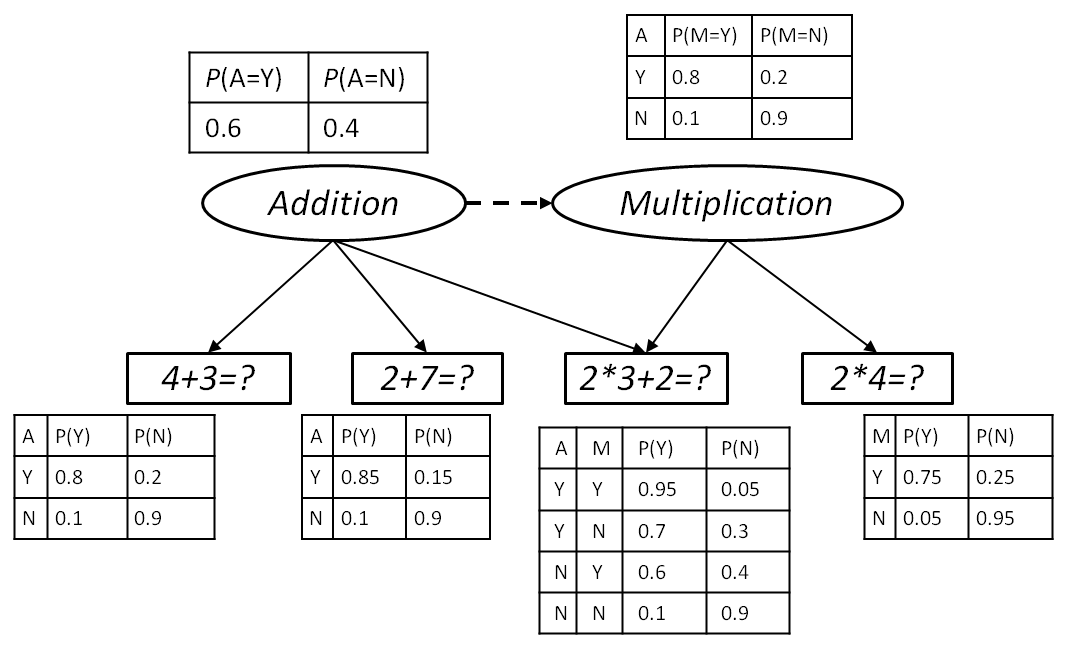
\includegraphics[width=.90\linewidth]{figures/studentmodel.png}
	\end{center}
	\vspace{-0.5em}
	\caption{A hypothetical Bayesian network. %learned with Algorithm~\ref{alg:COMMAND}. 
		Solid edges are given by item to skill mapping, dashed edges between skill variables are to be discovered from data.
		The conditional probability tables are to be learned.}
	\label{fig:smexample}
	\vspace{-1em} 
\end{figure}

Algorithm~\ref{alg:COMMAND} describes the COMMAND pipeline.
The input to COMMAND is a  matrix $\mathbf{D}$ with $n \times p$ dimensions,
representing $n$ students, answering $p$ items.
Each entry in $\mathbf{D}$ encodes the performance of a student (see Table~\ref{tbl:d-matrix} for an example).
Additionally, we require a $Q$-matrix to represent the item-to-skill mapping.
$Q$-matrices are often designed by subject matter experts but automatic methods to discover them exist~\cite{jp_aistats_2015}.
%, and (optionally) some constraints on what content can trigger a remediation.

%COMMAND first constructs the prerequisite relationships among the set of skills using constraints.
%Then, it  learns the parameters of a student model  that infers what skills a student has mastered.

\begin{table}[htb]\small
	\centering
	\caption{Example student performance matrix to use with COMMAND.  The performance of a student is encoded with 1 if the student answered correctly the item, and 0 otherwise. \label{tbl:d-matrix}}
	\begin{tabular}{@{}lllll@{}}
		\toprule
		User  & Item 1 & Item 2 & Item 3 & Item $p$ \\ \midrule
		Alice & 0      & 1      &        & 0        \\
		Bob   & 1      & 1      & ...    & 1        \\
		Carol & 0      & 0      &        & 1        \\
		\multicolumn{5}{c}{...}                     \\ \bottomrule
	\end{tabular}
\end{table}

\begin{algorithm}[!ht]
	\begin{algorithmic}[1]
		\Require A matrix $\mathbf{D}$ of student performance on a set of test items, skill-to-item mapping $Q$ (containing a set of skills $\mathbf{S}$).
		%and a set of constraints $\mathbf{C}$ reflecting experts' beliefs on the prerequisite structure
		\State  $G_0\leftarrow$ Initialize$(\mathbf{S}, Q)$ ~~~~~~~~~~~~~~~~\tikzmark{inittop}\tikzmark{right}
		\State $i\leftarrow 0$ \tikzmark{initbot}
		\Do \tikzmark{semtop}
		\State \emph{E}-step: 
		\State ~~~ $\Theta_i^*\leftarrow$ ParametricEM($G_i,\mathbf{D}$) 
		\State ~~~ $\mathbf{D}_i^*\leftarrow$ Inference($G_i,\Theta_i^*,\mathbf{D}$) 
		\State \emph{M}-step:
		\State ~~~ $\langle G_{i+1}, \Theta_{i+1}\rangle\leftarrow$ BNLearning($G_i$,$\mathbf{D}_i^*$)
		\State ~~~ $i\leftarrow i+1$
		\doWhile{stop criterion is not met}~~~~~~~~~~~~~~~~~~\tikzmark{right}\tikzmark{sembot}
		\State $RE\leftarrow FindReversibleEdges(G_i)$  ~~~~~~~~~~~~~~~~~~~~~\tikzmark{lsmtop}\tikzmark{right}
		\State $EC\leftarrow EnumEquivalentDAGs(G_i)$
		\State $DE\leftarrow \{\}$
		\For{every reversible edge $S_i - S_j$ in $RE$}
		%\State Compute $P(S_i=1|S_j=1)$, $P(S_j=0|S_i=0)$\\~~~~~$P(S_j=1|S_i=1)$ and $P(S_i=0|S_j=0)$
		%\LineComment {Can be computed using  Junction tree:}
		\State $ratio\leftarrow\frac{P(S_j=0|S_i=0)}{P(S_i=0|S_j=0)} $\footnote{}
		\If {$ratio\ge 1$}
		\State $ratio^*=ratio$
		\State $DE\leftarrow DE\cup S_i\rightarrow S_j$ 
		\Else
		\State $ratio^*=\frac{1}{ratio}$
		\State $DE\leftarrow DE\cup S_i\leftarrow S_j$
		\EndIf
		\EndFor
		\State $sort(DE)$ by $ratio^*$ in descending order
		\While{$DE$ is not empty}
		\State $e\leftarrow dequeue(DE)$
		\If{$\exists G\in EC$ $e\in G$}
		\State $\forall G\in EC$, remove $G$ from $EC$ if $e\notin G$
		\EndIf
		\EndWhile
		\State return $EC$
		\tikzmark{lsmbot}
	\end{algorithmic}
	\AddNote{inittop}{initbot}{right}{\footnotesize Initialization}
	\AddNote{semtop}{sembot}{right}{\footnotesize Structural EM}
	\AddNote{lsmtop}{lsmbot}{right}{\footnotesize Discriminate between equivalent BNs}
	\caption{The COMMAND algorithm  \label{alg:COMMAND}}
	\vspace{-1em}
\end{algorithm}
\footnotetext{$P(S_i=a|S_j=b)$ can be computed using any Bayesian network inference algorithm such as Junction tree algorithm\cite{koller2009probabilistic}.}

COMMAND relies on a popular machine learning algorithm called \textit{Structural Expectation Maximization} (Structural EM), 
which to the extent of our knowledge has not been used in educational applications before. 
Structural EM extends the Expectation Maximization (EM) algorithm to allow efficient structure learning of Bayesian networks 
when there are latent variables or missing values in the data.
%discovery of edges between nodes, and not just inferring the CPTs. 
%\hl{is this ok? a reviewer didn't get that Structural EM wasn't EM :-P}
A secondary contribution of our work is introducing Structural EM for learning Bayesian network structures from educational data.
We now describe the  steps of COMMAND in detail.

\subsection{Initial Bayesian Network}
\label{sec:initial_bn}
COMMAND first creates an initial Bayesian network using the  $Q$-matrix
% and a set of constraints reflecting experts' belief
%(step 1 of Algorithm~\ref{alg:remind}).
by creating an arc to each item from each of its required skills.
Because there are no edges between the skills, this  initial network does not encode any prerequisite information.
COMMAND uses Structural EM to learn arcs  (prerequisites) between the skill variables.

\subsection{Structural EM}
\label{sec:sem}

\begin{figure}%[!ht]
	\begin{center}
		%\framebox[4.0in]{$\;$}
		%\fbox{\rule[-.5cm]{0cm}{4cm} \rule[-.5cm]{4cm}{0cm}}
		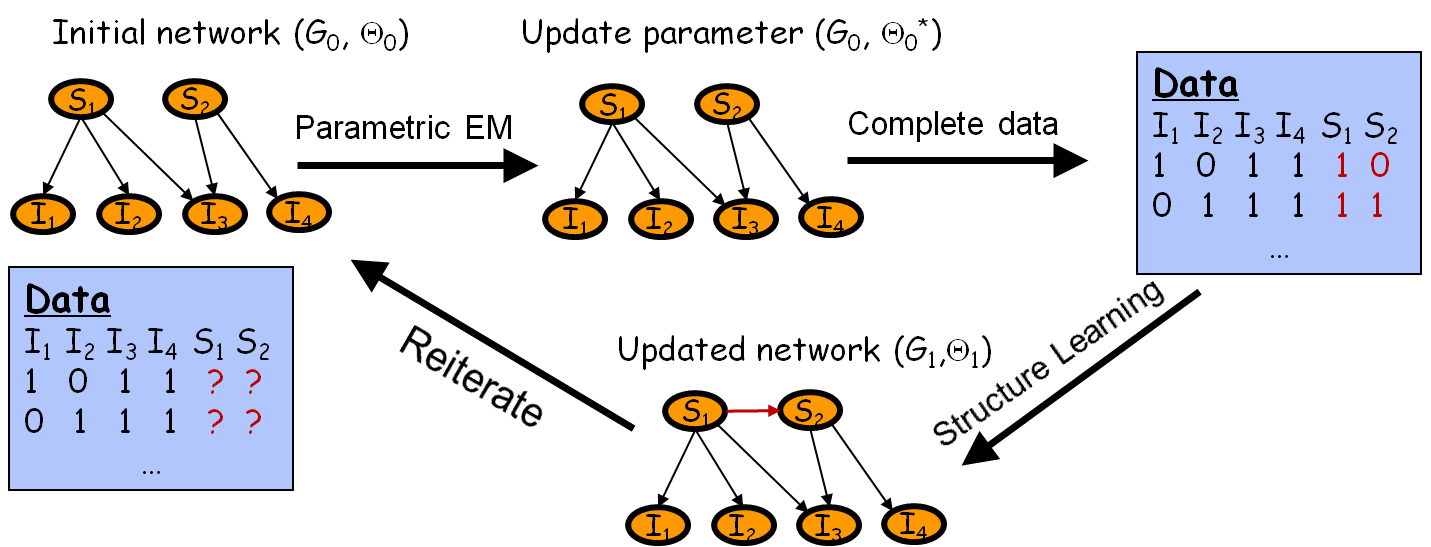
\includegraphics[width=1.0\linewidth]{figures/sem.png}
	\end{center}
	\caption{\small An illustration of the Structure EM algorithm to discover the structure of the latent variables. $G$ represents the DAG structure. $\Theta$ is the set of conditional probability tables (CPTs).}
	\label{fig:sem}
	\vspace{-1em} 
\end{figure} 

A common solution to learning a Bayesian network from data is the score-and-search approach \cite{cooper1992bayesian,heckerman1997bayesian}.
This approach uses a scoring function (like  the Bayesian Information Criterion (BIC)) to measure the fitness of a Bayesian network structure to the observed data, 
and it attempts to find the optimal model in the space of all possible Bayesian network structures.
However, the conventional score-and-search approaches rely on efficient computation of the scoring function, 
which is only feasible for problems where data contain observations for all variables in the Bayesian network.
Unfortunately, our domain has skill variables that are not directly observed.
An intuitive work-around is to use EM  to estimate the scoring function.
However, in this case EM takes a large number (hundreds) of iterations that require Bayesian network inference, which is computationally prohibitive.
Further, we need run EM for each candidate structure, and the number of possible Bayesian network structures is super-exponential with respect to the number of nodes.
The Structural EM algorithm \cite{friedman1997learning} is an efficient alternative.
%We now summarize how it works.

Structural EM is an iterative algorithm that  inputs a matrix $\mathbf{D}$ of student performance (see example Table~\ref{tbl:d-matrix}). %, where columns are the set of exercise items $\mathbf{I}$ and each row contains a student's performances on all these exercise items.
Figure~\ref{fig:sem} illustrates one iteration of the Structural EM algorithm. The relevant steps are also sketched in Algorithm~\ref{alg:COMMAND}. 
Each iteration consists of an Expectation step (\emph{E-step}) and a Maximization step (\emph{M-step}). 
%Structural EM calculates in each iteration a candidate model structure $G$ be by iterating over the Expectation and Maximization steps.
In the \emph{E-step}, it first finds the maximum likelihood estimate $\Theta^*$ of the CPTs 
for the current structure $G$ calculated from previous iteration using parametric EM. %\footnote{The first  network is created from the $Q$-matrix in the initialization step.}
It then does Bayesian inference to compute the expected values for the latent variables using the current model $(G,\Theta^*)$, 
and uses the values to complete the data.
In the \emph{M-step}, it uses the conventional score-and-search approach to optimize the structure according to the completed data (as if the latent variables were observed).
Since the space of possible Bayesian network structures is super-exponential, 
exhaustive search is intractable and local search algorithms, such as greedy hill-climbing search, are often used.
The \emph{E-step} and \emph{M-step} interleave and iterate until some stop criterion is met, e.g., the scoring function does not change significantly.
Contrast to the conventional score-and-search algorithm, Structural EM runs EM only on one structure in each iteration, thus is computationally more efficient.

We use an efficient implementation of Structural EM available online called LibB\footnote{\url{http://compbio.cs.huji.ac.il/LibB/programs.html}}.
Because COMMAND's initialization step
%REMIND's implementation of prerequisite discovery we use Structural EM to learn the arcs between skills, but 
fixes the arcs from skills to items according to the ${Q}$-matrix,
%For this, we initialize the network as $G_0$ where skill variables and item variables are connected according to the ${Q}$-matrix, but skill variables are disconnected with each other. 
the \emph{M-step} only needs to consider the candidate structures that comply with the ${Q}$-matrix.
%We believe that this reduction of the space of candidate models improves efficiency. %makes the Structural EM more efficient.
An advantage of using Structural EM to discover the prerequisite relationship of skills is that it can be easily extended to incorporate domain knowledge.
For example, we can  place constraints on the output structure to force or to disallow a skill to be a prerequisite of another skill.
Another advantage of Structural EM is that it can be applied when there are missing data in the student performance matrix $\mathbf{D}$~\cite{friedman1997learning}. 
That is, some students do not answer all the items.
% This ``missing values" problem is very common in real-world situations.
%Structural EM can be applied to this type of data since it was originally developed to solve the "missing values" problem.
The general idea is, in the \emph{E-step}, the algorithm also computes the expected values for missing data points, in addition for latent variables. 

%Consider, an intelligent tutor that teaches the content of a book. 
%The book content structure provides a natural ordering of the chapters. 
%We may use the book structure to engineer domain knowledge that an introductory chapter cannot be prerequisite of content that appears later in the book.


\subsection{Discriminate Between Equivalent BNs}
\label{sec:discriminatebns}

Structural EM selects a Bayesian network model based on how well it explains the distribution of the data. 
Bayesian network theory states that some Bayesian networks are statistically equivalent in representing the data.
Thus, the output from Structural EM is actually an equivalence class (EC) that may contain many Bayesian network structures\footnote{Structural EM outputs a DAG. However,  the scoring function  does not discriminate between the many DAGs of the equivalence class.}.
These equivalent Bayesian networks have the same skeleton and the same $v$-structures\footnote{A $v$-structure with nodes $u,v,w$ in a DAG are the directed edges $u\rightarrow v$ and $w\rightarrow v$ and $u$ and $w$ are not adjacent in the DAG~\cite{verma1990equivalence}.}. 
For instance, Figure~\ref{fig:equivnets} gives an example of a simple equivalence class containing three Bayesian networks 
that are not distinguishable by Structural EM algorithm and the method in \cite{scheines2014discovering}.
They share the skeleton but differ in the orientation of at least one of the edges (we will call such an edge a reversible edge). 
They apparently represent three different prerequisite structures.

	\begin{figure}[!ht]\small
		\centering
		\begin{subfigure}[t]{0.32\linewidth}
			\centering
			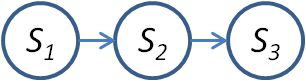
\includegraphics[width=0.9\linewidth]{figures/s1s2s3.png}
			\caption{\label{fig:equivnet1}}
		\end{subfigure}
		\begin{subfigure}[t]{0.32\linewidth}
			\centering
			
\includegraphics[width=0.9\linewidth]{figures/s2s1s3.png}
			\caption{\label{fig:equivnet2}}
		\end{subfigure}
		\begin{subfigure}[t]{0.32\linewidth}
			\centering
			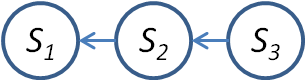
\includegraphics[width=0.9\linewidth]{figures/s3s2s1.png}
			\caption{\label{fig:equivnet3}}			
		\end{subfigure}		
		\caption{Three equivalent Bayesian networks representing different prerequisite structures.\label{fig:equivnets} }
	\end{figure}
	
	
\subsubsection{Domain Knowledge}
\label{sec:usedomain}
To determine a unique structure, we use a heuristic based in domain knowledge to determine the orientation of each reversible edge.
For convenience in notation, let's assume that the random variables that represent skill proficiency can take two values: 0 if the skills is not mastered, and 1 if the skill is mastered.
Our assumption is that if a skill $S_1$ is the prerequisite of a skill $S_2$, a student can not master skill $S_2$ before she masters $S_1$.
More formally:

\textbf{Assumption.} If $S_1$ is a prerequisite of $S_2$ (i.e., $S_1\rightarrow S_2$), then $S_1=0\Rightarrow S_2=0 $. %, which is equivalent to $S_2=1\Rightarrow S_1=1$.
In other words, $P(S_2=\text{0}|S_1=0)=1$.

Our assumption implies  that  $S_1$ cannot be a prerequisite of $S_2$ if $P(S_2=0|S_1=0)=1$ does not hold.
This puts a constraint on the joint distribution encoded by the Bayesian network to be learned.


%For this purpose, we propose to use the following domain knowledge.

%\textbf{Knowledge 1}. If $S_1$ is a prerequisite of $S_2$, i.e., $S_1\rightarrow S_2$, then $P(S_1=1|S_2=1)= 1$ and $P(S_2=0|S_1=0)= 1$.
%
%\textbf{Knowledge 1} says if a skill $S_1$ is the prerequisite of a skill $S_2$,
%a student must master skill $S_1$ before he masters $S_2$ and it is impossible for him to master $S_2$ if he has not mastered $S_1$.
%In other words, $S_1$ is not a prerequisite of $S_2$ if at least one of the conditions does not hold.
%This puts a constraint on the joint distribution encoded by the Bayesian network to be learned.
%We can check for any reversible edge $S_1-S_2$ in the Bayesian network, either $P(S_1=1|S_2=1)= 1$ and $P(S_2=0|S_1=0)= 1$, or $P(S_2=1|S_1=1)= 1$ and $P(S_1=0|S_2=0)= 1$. 
%If the former holds, $S_1\rightarrow S_2$; otherwise, $S_1\leftarrow S_2$.  
%However, in real situations, it is possible for a student to master the post-requisite even he does not know the prerequisite. 
%Further, there is always noise in the data. Thus, the two conditional probabilities $P(S_1=1|S_2=1)$ and $P(S_2=0|S_1=0)$ are not exactly but close to 1.
%Thus, we use the following empirical rule: if $P(S_1=1|S_2=1)\cdot P(S_2=0|S_1=0)\ge P(S_2=1|S_1=1)\cdot P(S_1=0|S_2=0)$, we determine $S_1\rightarrow S_2$; 
%otherwise, we determine $S_1\leftarrow S_2$.
%Note that these conditional probabilities can be computed easily from the Bayesian network model output from Structural EM. 
%The intuition behind this is that the two probabilities $P(S_1=1|S_2=1)$ and $P(S_2=0|S_1=0)$ are certificates of the prerequisite structure $S_1\rightarrow S_2$.
%The larger of these two probabilities, the more likely the relationship $S_1\rightarrow S_2$ holds.
%Since here we are concerned with which direction the edge goes, we simply compare the products of two probabilities and select the direction that is more probable. 



%If $S_1$ is a prerequisite of $S_2$, i.e., $S_1\rightarrow S_2$, then $P(S_1=1|S_2=1)= 1$ and $P(S_2=0|S_1=0)= 1$.
%We can check for any reversible edge $S_1-S_2$ in the Bayesian network, either $P(S_2=0|S_1=0)=1$ or $P(S_1=0|S_2=0)= 1$. 
%If the former holds, $S_1\rightarrow S_2$; otherwise, $S_1\leftarrow S_2$.\footnote{$P(S_2=0|S_1=0)=1$ and $P(S_1=0|S_2=0)= 1$ can hold simultaneously under the condition
%that} 
For example, consider the case of choosing the orientation of a reversible edge $S_1 - S_2$ from $S_1 \leftarrow S_2$ or  $S_1 \rightarrow S_2$.
We can check whether $P(S_2=0|S_1=0)=1$ or $P(S_1=0|S_2=0)=1$.
However, it is possible that our assumption does not hold, and a student got to master a skill even if he does not know the prerequisite. 
Moreover, because of statistical noise,  the conditional probability $P(S_2=0|S_1=0)$ may not  be exactly 1.
Thus, we use the following empirical rule: 

\textbf{Rule 1}. if $P(S_2=0|S_1=0)\ge P(S_1=0|S_2=0)$, we determine $S_1\rightarrow S_2$; otherwise, we determine $S_1\leftarrow S_2$.

Note that these two conditional probabilities can be computed easily from the Bayesian network model output from Structural EM. 
The intuition behind this rule is that the conditional probability $P(S_2=0|S_1=0)$ can be interpreted as the strength of the prerequisite relationship $S_1\rightarrow S_2$.
The larger of this probability, the more likely the relationship $S_1\rightarrow S_2$ holds.
Since here we are concerned with which direction the edge goes, we simply compare the two probabilities and select the direction that is more probable. 
Note  that $P(S_2=0|S_1=0)=1$ and $P(S_1=0|S_2=0)=1$ may hold simultaneously. 
If $S_1\rightarrow S_2$ is true, $P(S_1=0|S_2=0)=1$ only if $P(S_1=1)=0$ or if $P(S_2=0|S_1=1)=0$.\footnote{Since $P(S_1=0|S_2=0)=\frac{P(S_2=0|S_1=0)P(S_1=0)}{P(S_2=0|S_1=0)P(S_1=0)+P(S_2=0|S_1=1)P(S_1=1)}$, $P(S_1=0|S_2=0)=1$ only if $P(S_2=0|S_1=1)P(S_1=1)=0$.} 
If $P(S_1=1)=0$, this implies that no student knows $S_1$. 
If $P(S_2=0|S_1=1)=0$, it means that learning $S_2$ becomes trivial once students know $S_1$. 
For simplicity, we ignore this extreme case.


\subsubsection{Theoretical Justification of Heuristic}
\label{sec:theory}

We now provide theoretical justification for the  rule we  propose.
%We consider the simple Bayesian network in Figure~\ref{fig:equivnet1}, which has only one reversible edge $S_1-S_2$.
%This model has three free conditional probability parameters: $P(S_1=0)=p$, $P(S_2=0|S_1=0)=q$, $P(S_2=1|S_1=1)=r$.
%If we observe data generated from this model, 
%can we use the rule to determine $S_1\rightarrow S_2$? %by comparing $P(S_1=1|S_2=1)\cdot P(S_2=0|S_1=0)$ and $P(S_2=1|S_1=1)\cdot P(S_1=0|S_2=0)$?
%Equivalently, we use rule $ratio=\frac{P(S_1=1|S_2=1)\cdot P(S_2=0|S_1=0)}{P(S_2=1|S_1=1)\cdot P(S_1=0|S_2=0)}\ge 1$.
%Using Bayes rule and rules of probability, the rule becomes
%\begin{align}
%ratio=\frac{(1-p)(qp+1-r-p+pr)}{p[r(1-p)+p(1-q)]}\ge 1,
%\end{align}
%which can be simplified to
%\begin{align}
%\frac{(1-p)(1-r)-p(1-q)}{p[r(1-p)+p(1-q)]}\ge 0.
%\end{align}
%
%The rule holds only if $(1-p)(1-r)-p(1-q)\ge 0$. Thus, we can use the rule to determine $S_1\rightarrow S_2$ if $(1-p)(1-r)-p(1-q)\ge 0$.
%Since $ratio$ depends on $p$, $q$ and $r$, we study how $ratio$ changes with these parameters.
%Figure~\ref{fig:contours} shows the contour plots of $log(ratio)$ against $P(S_1=0)$ and $P(S_2=1|S_1=1)$ for three different values of $P(S_2=0|S_1=0)$.
%The white region in each contour plot is the region where the rule is not applicable. 
%That is, in this region, $ratio<1$ even $S_1\rightarrow S_2$ is the true model.
%As it is showed, if $P(S_2=0|S_1=0)=q=1$, 
%the rule is always applicable no matter what values $P(S_1=0)$ and $P(S_2=1|S_1=1)$ are.
%With $P(S_2=0|S_1=0)$ decreasing, the white region becomes larger and the rule becomes more inapplicable.
%$P(S_2=0|S_1=0)$ can be interpreted as the strength of the prerequisite relationship. When the prerequisite relationship is weaker, the rule is less applicable 
%and using the rule to determine the prerequisite relationship is less accurate.
Consider a simple equivalence class, which contains two equivalent DAGs $S_1\rightarrow S_2$ and $S_1\leftarrow S_2$, where the true model is $S_1\rightarrow S_2$.
We have three free conditional probability parameters: $P(S_1=0)=p$, $P(S_2=0|S_1=0)=q$, $P(S_2=1|S_1=1)=r$.
%by comparing $P(S_1=1|S_2=1)\cdot P(S_2=0|S_1=0)$ and $P(S_2=1|S_1=1)\cdot P(S_1=0|S_2=0)$?
%How can we use data to If we observe data generated from this model, can we use the rule to discriminate between $S_1\rightarrow S_2$ and $S_1\leftarrow S_2$? 
Let's define a \textit{ratio} that quantifies choosing the true model:
\begin{align}
ratio=\frac{P(S_2=0|S_1=0)}{P(S_1=0|S_2=0)}.
\end{align}
Using Bayes rule and rules of probability, the rule $ratio\ge 1$ becomes $(1-p)(1-r)-p(1-q)\ge 0$.
Since \textit{ratio} depends on $p$, $q$ and $r$, we study how $ratio$ changes with these parameters.
Figure~\ref{fig:contours} shows the contour plots of $log(ratio)$ against $P(S_1=0)$ and $P(S_2=1|S_1=1)$ for three different values of $P(S_2=0|S_1=0)$.
The white region in each contour plot is the region where our heuristic fails  because $ratio<1$. % $S_1\rightarrow S_2$ is the true model.
Figure~\ref{fig:contours}(a) shows that when $P(S_2=0|S_1=0)=q=1$, our heuristic rule is always correct, no matter what, because there is no white space. % values $P(S_1=0)$ and $P(S_2=1|S_1=1)$ take \hl{how does the graph show this??}.
With $P(S_2=0|S_1=0)$ decreasing, the white region becomes larger and the rule becomes less accurate.
As mentioned, $P(S_2=0|S_1=0)$ can be interpreted as the strength of the prerequisite relationship. 
If we fix the value of $P(S_2=0|S_1=0)$ and assume that the two free parameters $p$ and $r$ are independent and uniformly distributed, then the area of the white region represents the probability that the rule makes a wrong decision.
As the strength of the prerequisite relationship  gets weaker, our  rule to determine the prerequisite relationship becomes less accurate.



	
		\begin{figure}[!ht]\small
			\centering
			\begin{subfigure}[t]{0.32\linewidth}
				\centering
				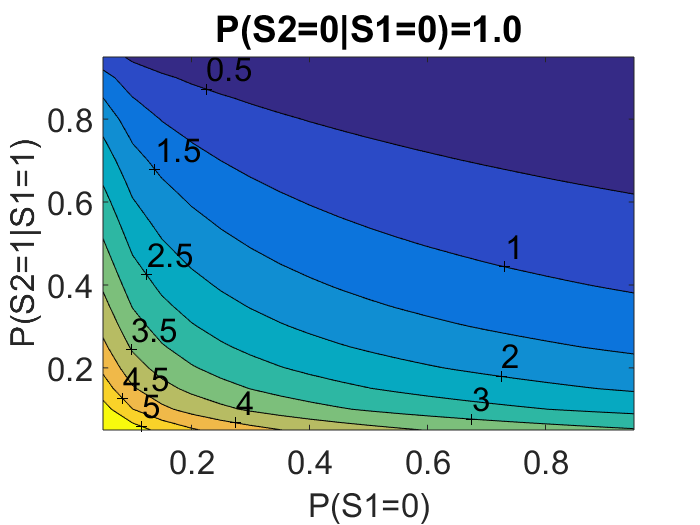
\includegraphics[width=1.05\linewidth]{figures/contour1.png}
				\caption{\label{fig:contour1}}
			\end{subfigure}
			\begin{subfigure}[t]{0.32\linewidth}
				\centering
				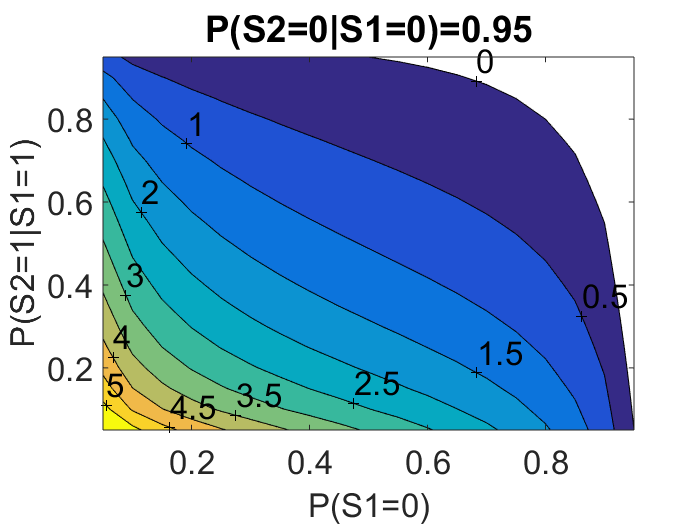
\includegraphics[width=1.05\linewidth]{figures/contour2.png}
				\caption{\label{fig:contour2}}
			\end{subfigure}
			\begin{subfigure}[t]{0.32\linewidth}
				\centering
				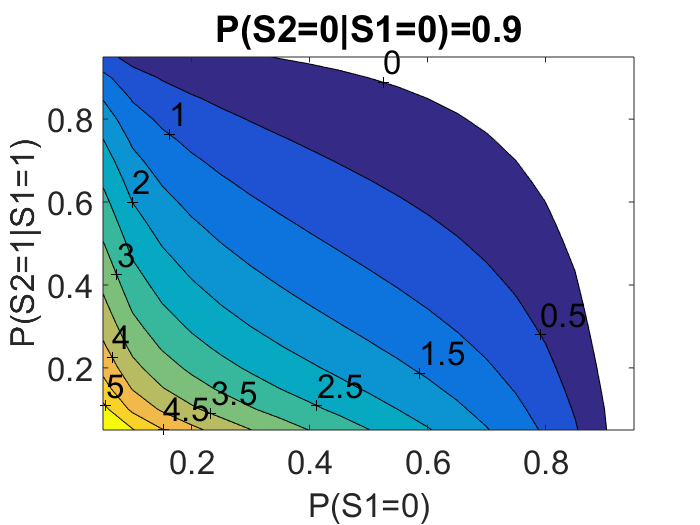
\includegraphics[width=1.05\linewidth]{figures/contour3.png}
				\caption{\label{fig:contour3}}
			\end{subfigure}						
			\caption{Contour plots of $log(ratio)$ against $P(S_1=0)$ and $P(S_2=1|S_1=1)$ for various values of $P(S_2=0|S_1=0)$.\label{fig:contours} }
			\vspace{-1em}
		\end{figure}
		
\subsubsection{Orient All Reversible Edges}
Using our proposed rule, we can orient every reversible edge in the network structure. 
However, orienting each reversible edge is not independent and may conflict with each other.
Having oriented one edge would constrain the orientation of other reversible edges because we have to ensure the graph is a DAG and the equivalence property is not violated.
For example, in Figure~\ref{fig:syn-nets}a, if we have determined $S_1\rightarrow S_2$, the edge $S_2\rightarrow S_3$ is enforced.
In this paper, we take an ad-hoc strategy to determine the orientation for all reversible edges. 
For each reversible edge $S_i-S_j$, we let $ratio^*=ratio$ if $ratio \ge 1$ and $ratio^*=\frac{1}{ratio}$ otherwise. 
The larger the $ratio^*$ is, the more confidently when we decide the orientation.
We sort the list of reversible edges by $ratio^*$ in descending order. We then orient the edges by this ordering.
%When one edge is oriented, the constraint is propagated to other reversible edges.
%That is, for any of the remaining reversible edges, 
%\hl{<- how do this different procedures differ? ->}
In our implementation, we use the following strategy: 
we first enumerate all equivalent Bayesian networks and make them a list of candidates; 
when an edge is oriented to $S_i\rightarrow S_j$, we remove all contradicting Bayesian networks from the list.
Eventually only one Bayesian network structure stands. This procedure is detailed in the \emph{Discriminate between equivalent BNs} section of Algorithm~\ref{alg:COMMAND}.  
The $EnumEquivalentDAGs(G_i)$ implements the algorithm of enumerating equivalent DAGs in \cite{chen2014finding}.

%\newpage
\section{Evaluation}
In \S~\ref{sec:synthetic}, we evaluate COMMAND with simulated data  to assess the quality of the discovered prerequisite structures.
Then, in \S~\ref{sec:real} we use  data collected from real students.
In all our experiments, we use BIC as the scoring function in Structural EM . 
%The BIC score for a Bayesian network model is composed of a likelihood term and a term to penalize the model complexity.

	\subsection{Simulated Data}
	\label{sec:synthetic}
	%We first use synthetic data to demonstrate the capability of Structural EM in learning the prerequisite structure of latent skill variables.
	%By using 
	%various factors, including sample size, number of skill or item variables, prior knowledge, noises in the data, 
	%affect the learning performance.
	
	Synthetic data allow us to study how COMMAND compares to the ground truth.
	For this, we engineered three prerequisite structures (DAGs), shown in Figure~\ref{fig:syn-nets}.
	Here, each figure represents different causal relations between the simulated latent skill variables.
	%Note that some edges are reversible and represented as undirected edges. 
	%Given observational data, the direction of some edges cannot be determined because the edges are \emph{reversible}%
	%We represent these edges as undirected lines.
	
	\begin{figure}[!ht]
		%\begin{center}
		\begin{minipage}[b]{0.45\linewidth}
			\centering
			
\includegraphics[width=0.9\linewidth]{figures/model1.png}\\~\\
			(a) Structure 1~\\~\\~\\
			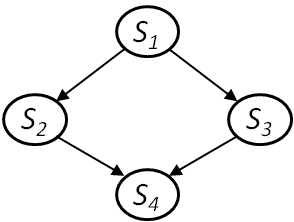
\includegraphics[width=0.8\linewidth]{figures/model2.png}\\~\\
			(b) Structure 2
		\end{minipage}
		\quad
		\begin{minipage}[b]{0.45\linewidth}
			\centering
			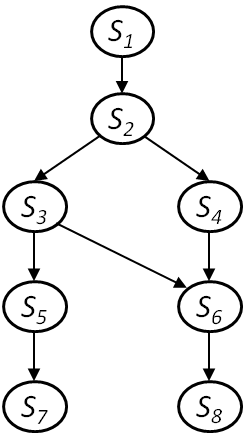
\includegraphics[width=0.7\linewidth]{figures/model3.png}\\~\\
			(c) Structure 3
		\end{minipage}	
		\caption{Three different DAGs between latent skill variables.  Item nodes are omitted.}
		\label{fig:syn-nets}
		%\vspace{-1em}
		%\end{center} 
	\end{figure} 
	
	For clarity, Figure~\ref{fig:syn-nets}  omits the item nodes;
	but each skill node is parent of six item variables and each item variable has 1-3 skill nodes as parents.
	All of these nodes are modeled using binary random variables.
	More precisely, the latent  nodes represent whether the student  achieves mastery of the skill,
	and the observed nodes indicate if the student answers the item correctly.
	Notice that these networks include the prerequisite structures as well as the skill-item mapping.
	
	We consider simulated data with different number of observations ($n=150, 500, 1000, 2000$).
	For each sample size and each  DAG, we generate ten different sets of conditional probability tables
	randomly with three constraints.
	First, we enforce that achieving mastery of the prerequisites of a skill will increase the likelihood of mastering the skill.
	Second, for each prerequisite pair $S_i\rightarrow S_j$,  $P(S_j=0|S_i=0)$ is randomly selected to be in $[0.9, 1.0]$.
	Finally, mastery of a skill increases the probability of student correctly answering the test item. 
	In total we generated 120 synthetic datasets (3 DAGs x 4 sample sizes x 10 CPTs), and  report the average results.
	
	
	We evaluate how well COMMAND can discover the true prerequisite structure using metrics designed to evaluate Bayesian networks structure discovery.
	In particular, we use the $F_1$ \emph{adjacency score} and the $F_1$ \emph{orientation score}.
	The adjacency score measures how well we can recover connections between nodes.
	It is a weighted average of the true positive adjacency rate and the true discovery adjacency rate.
	On the other hand, the orientation score measures how well we can recover the direction of the edges.
	%To measure the accuracy of edge orientation, we compute the $F_1$ \emph{orientation score}, 
	It is calculated as a weighted average of the true positive orientation rate and true discovery orientation rate.
	%This metric does not account for the directionality incorrect edges that are reversible.
	In both cases, the $F_1$ score reaches its best value at 1 and worst at 0. 
	Moreover, for comparison, we compute the $F_1$ \emph{adjacency score} for Bayesian network structures whose skill nodes are fully connected with each other. 
	These fully connected DAGs will serve as baselines for evaluating the adjacency discovery\footnote{We do not compute $F_1$ orientation score for fully connected DAGs because all edges in a fully connected DAG are reversible.}.
	For completeness, we list these formulas in tables~\ref{tbl:ar}~and~\ref{tbl:or}, respectively.
	
	
	% Please add the following required packages to your document preamble:
	% \usepackage{booktabs}
	\begin{table}[ht]
		\centering
		\caption{Formulas for measuring adjacency rate (AR) \label{tbl:ar}}
		\label{my-label}
		\begin{tabular}{@{}ll@{}}
			\toprule
			Metric & Formula \\ \midrule
			True positive    (\emph{TPAR}) & $\frac{ \text{\# of correct adjacencies in learned model} } { \text{ \# of adjacencies in true model} }$  \\
			True discovery (\emph{TDAR}) &  $\frac{ \text{\# of correct adjacencies in learned model} } { \text{ \# of adjacencies in learned model} }$ \\
			$F_1$-\textit{AR} &  $\frac{2\cdot \text{\emph{TPAR}} \cdot \text{\emph{TDAR}}} {\text{\emph{TPAR}}+\text{\emph{TDAR}}}$  \\
			\bottomrule
		\end{tabular}
	\end{table}
	
	
	\begin{table}[ht]
		\centering
		\caption{Formulas for measuring orientation rate (OR) \label{tbl:or}}
		\label{my-label}
		\begin{tabular}{@{}ll@{}}
			\toprule
			Metric & Formula \\ \midrule
			True positive  (\emph{TPOR}) & $\frac{ \text{\# of correctly directed edges in learned model} } {\text{ \# of directed edges in true model}}$  \\
			True discovery   (\emph{TDOR})& $\frac{ \text{\# of correctly directed edges in learned model } }{\text{ \# of directed edges in learned model}} $\\
			$F_1$-\textit{OR} &  $\frac{  2\cdot \text{\emph{TPOR}} \cdot \text{\emph{TDOR}} }{\text{\emph{TPOR}}+\text{\emph{TDOR}}}$ \\
			\bottomrule
		\end{tabular}
	\end{table}
	
	We use these metrics to evaluate the effect of varying the  number of observations  of the training set (sample size) on the quality of learning the prerequisite structure.
	We designed experiments to specifically answer the following four questions:
	\begin{enumerate}[noitemsep,topsep=2pt,parsep=0pt,partopsep=0pt]
		\item How does the type of items affect COMMAND's ability to recover the prerequisite structure?
		We consider the situation where in the model each item requires only one skill and the situation where each item requires multiple skills. 
		\item How well does COMMAND perform when there is noise in the data?
		We focus on studying noise due to the presence of unaccounted latent variables.
		\item How well does COMMAND perform when the student performance data have missing values?
		\item How is COMMAND compared with other prerequisite discovery methods?
		In particular, we compare COMMAND to the Probabilistic Association Rules Mining (PARM) method \cite{chen2015discovering}.
	\end{enumerate}
	We now investigate these questions.


	\subsubsection{Single-skill vs Multi-skill Items}
	
	We consider two situations where different types of $Q$-matrix are used. In the first situation,
	each item node maps to exactly one skill node. In the second one, each item maps to 1-3 skills. 
	Figure~\ref{fig:f1-single-multi} compares the $F_1$ of adjacency discovery and edge orientation results under the two types of $Q$-matrices.
	With only 500 observations, COMMAND improves on a fully connected Bayesian network baseline.
	COMMAND's  accuracy improves with the amount of data, but its accuracy is slightly lower when the $Q$-matrix contains items that require more than one skill. % than single-skill $Q$-matrix.
	A possible explanation for this is that multi-skill items may introduce more spurious correlations in the data.
	With just 2000 observations, COMMAND  recovers the true structures almost perfectly.
	
	\begin{figure}[ht]
		\begin{center}
			\begin{tabular}{>{\centering}m{1.5in} >{\centering\arraybackslash}m{1.5in}}
				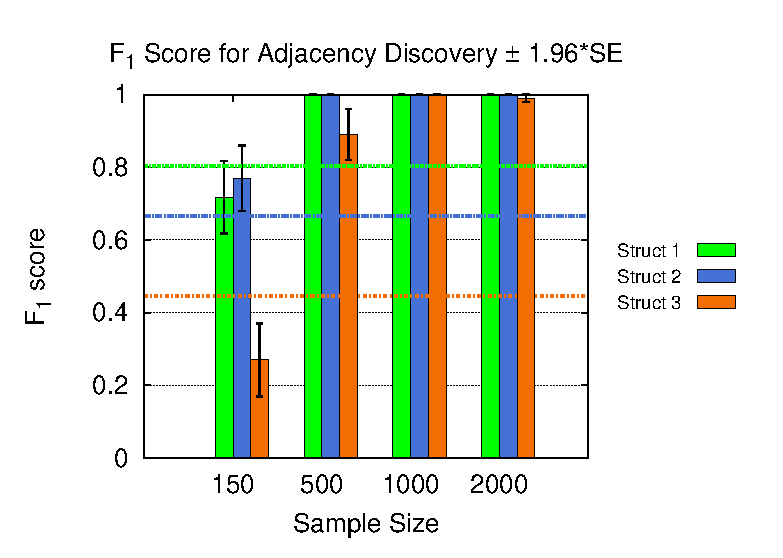
\includegraphics[width=1.1\linewidth]{figures/F1A_single.eps} &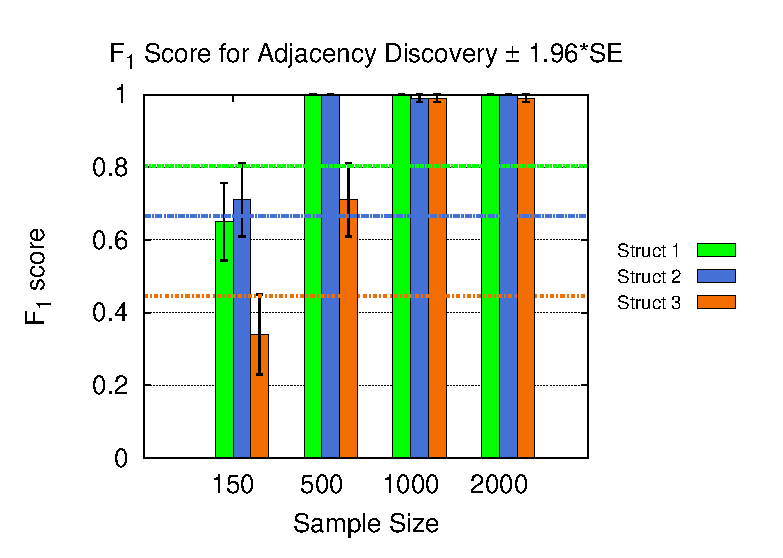
\includegraphics[width=1.1\linewidth]{figures/F1A_multi.eps}\\
				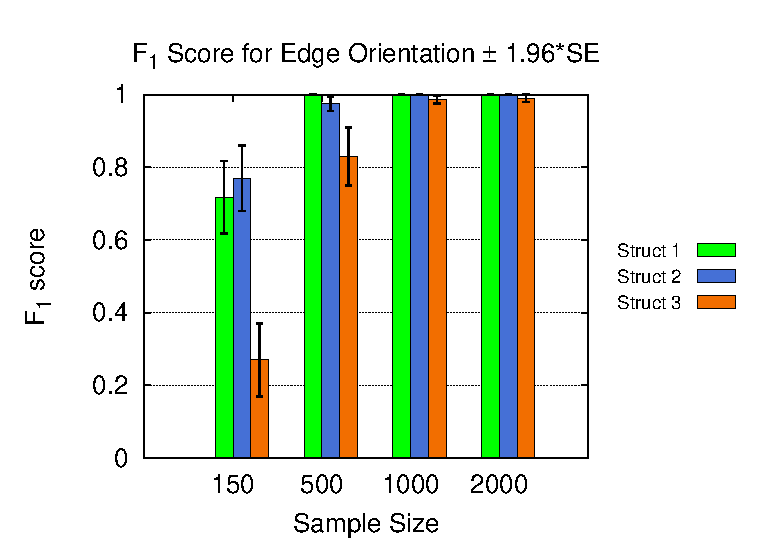
\includegraphics[width=1.1\linewidth]{figures/F1O_single.eps} &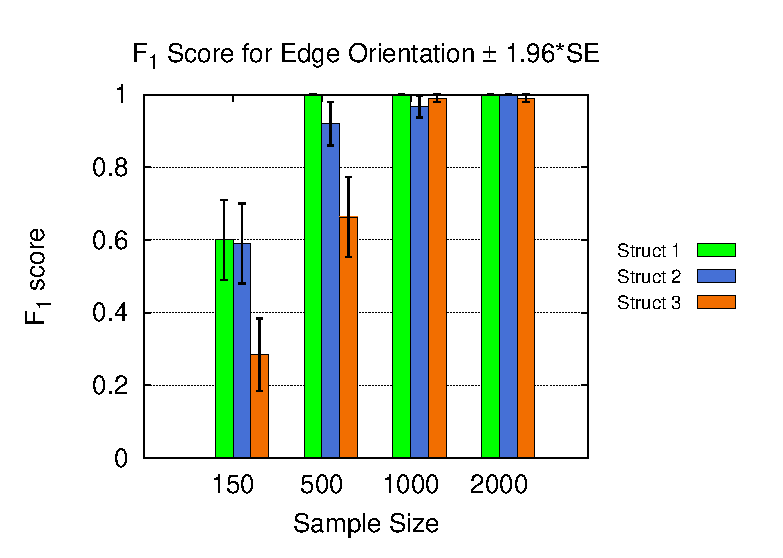
\includegraphics[width=1.1\linewidth]{figures/F1O_multi.eps}\\
				Single Skill& Multiple Skill
			\end{tabular}
		\end{center}
		\vspace{-1em}
		\caption{Comparison of $F_1$ scores for adjacency discovery (top row) and for edge orientation (bottom row). 
			Horizontal lines are baseline scores for fully-connected (complete) networks.
			The error bars show the $95\%$ confidence intervals, i.e., $\pm 1.96*$\texttt{SE}.} 
		\label{fig:f1-single-multi}
		%\vspace{-1em}
	\end{figure} 

	
	\subsubsection{Sensitivity to Noise}	
	
	%\hl{Hard to read}
	Real-world data sets often contain various types of noise.
	For example,  noise may occur due to latent variables that are not explicitly modeled. 
	%For example, students' performances in a test also depends on their individual ability (in addition to their mastery status of the required skills). 
	%This will create noises in the data if we don't directly model the student's ability.
	To evaluate the sensitivity of COMMAND to noise, we synthesize the three Bayesian networks in Figure~\ref{fig:syn-nets} to include a \emph{StudentAbility} node 
	that takes three possible states (low/med/high). 
	In these Bayesian networks, students' performance depends not only on whether they have mastered the skills, but also on their individual ability. % (in addition to their mastery status of the required skills).
	For simplicity, all items in the setting are single-skilled items. 
	We first simulated data from  Bayesian networks that have a \emph{StudentAbility} variable to generate ``noisy'' data samples, and 
	%There is an arc from \emph{StudentAbility} to each item variable in these data generating models. 
	then use this data to recover the prerequisite structure. % from these truncated data samples. 
	Figure~\ref{fig:stuabilitymodel} illustrates the procedure of this sensitivity analysis experiment for Structure 1.
	
			\begin{figure}[ht]
				\begin{center}
					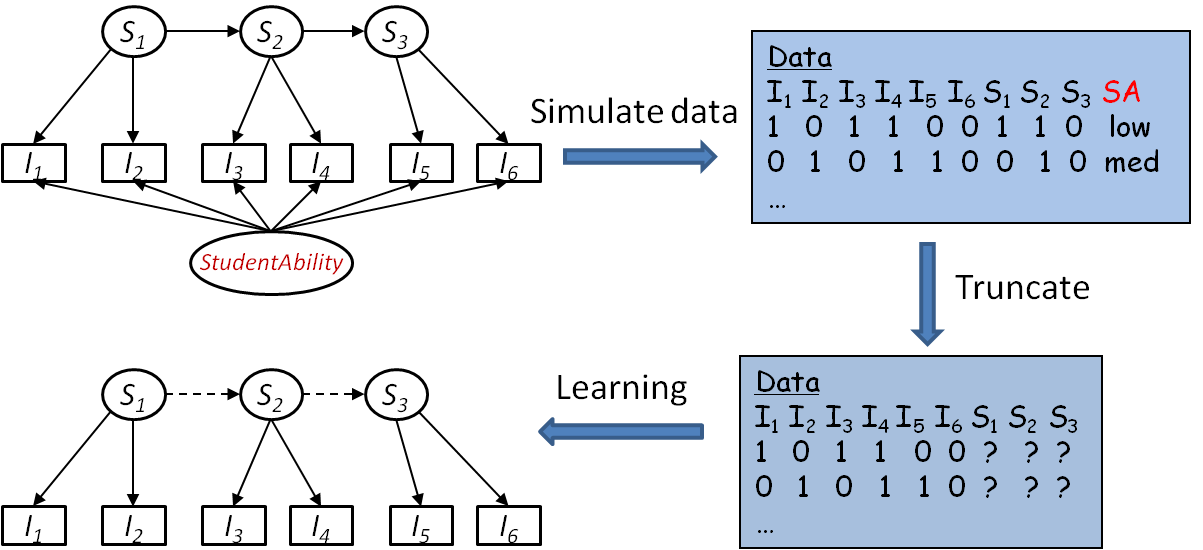
\includegraphics[width=.95\linewidth]{figures/studentability.png}
				\end{center}
				\vspace{-1em}
				\caption{Evaluation of COMMAND with noisy data} 
				\label{fig:stuabilitymodel}
			\end{figure}
			
			\begin{figure}[!ht]
				\begin{center}
					\centering
					\begin{tabular}{>{\centering}m{1.5in} >{\centering\arraybackslash}m{1.5in}}
						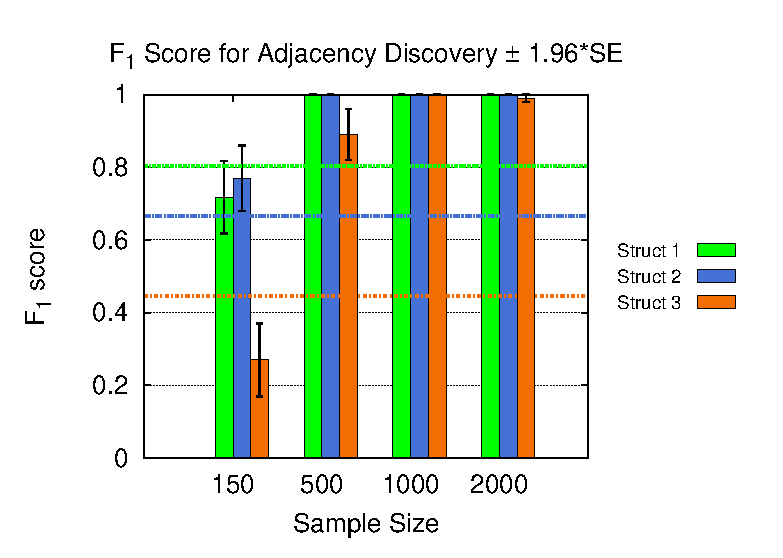
\includegraphics[width=1.1\linewidth]{figures/F1A_single.eps} &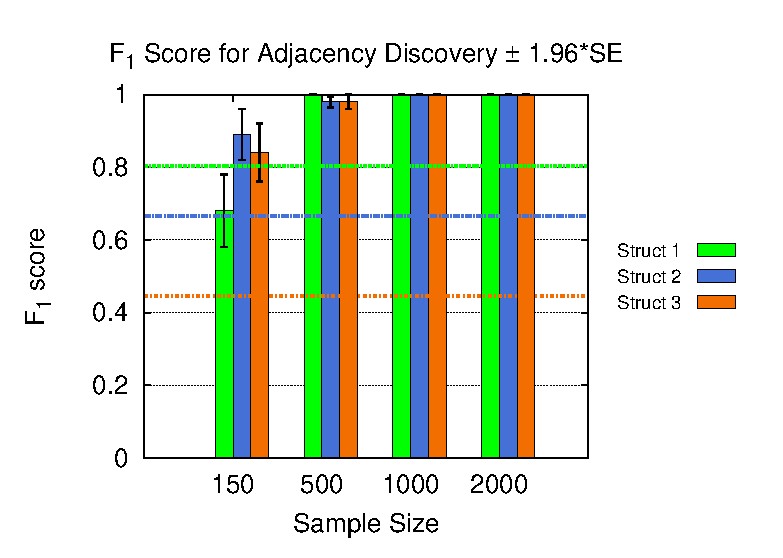
\includegraphics[width=1.1\linewidth]{figures/F1A_single_noisy.eps}\\
						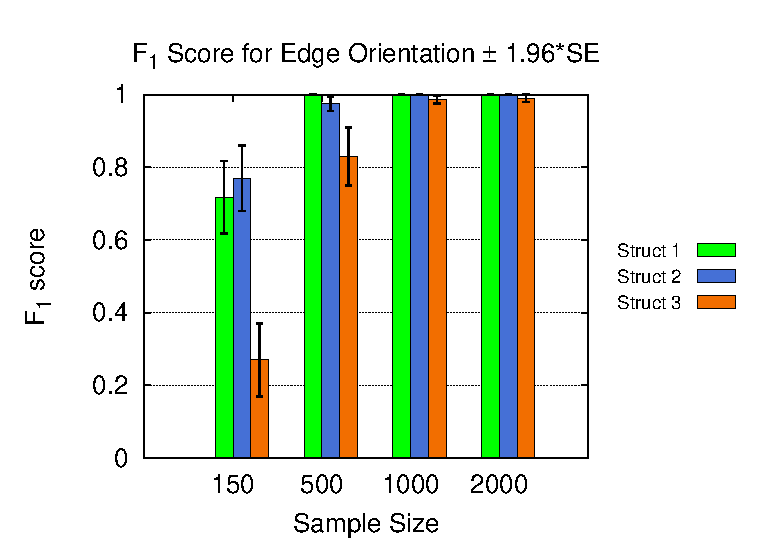
\includegraphics[width=1.1\linewidth]{figures/F1O_single.eps} &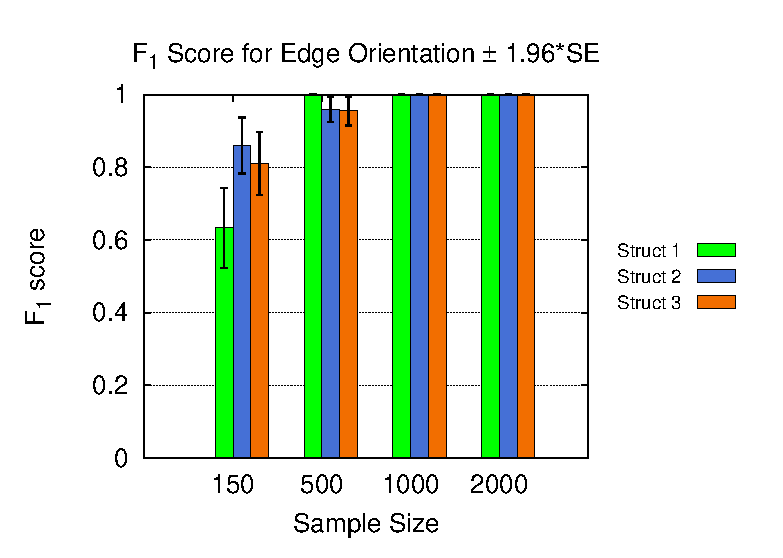
\includegraphics[width=1.1\linewidth]{figures/F1O_single_noisy.eps}\\
						No Noise & Noisy
					\end{tabular}
				\end{center}
				\vspace{-1em}
				\caption{Results of adding systematic noise. Top: Comparison of $F_1$ scores for adjacency discovery. Horizontal lines are baseline $F_1$ scores computed for fully connected Bayesian networks. Bottom: Comparison of $F_1$ scores for edge orientation. }
				\label{fig:f1-noisy} 
			\end{figure}

		
	
	Figure~\ref{fig:f1-noisy} compares the results where noise was introduced or not.
	Interestingly, the noise  actually improves COMMAND's  accuracy.
	This improvement is more evident when the sample size is small (see $n=150$).
	%We hypothesize that adding this variable is actually removing noise by separating students by ability, which can help the structure learning.
	For smaller sample sizes, Structural EM usually discovers less relationships than actually exist, because BIC prefers sparse structures.
	We hypothesize that the correlations caused by \emph{StudentAbility} node would cause Structural EM to add ``stronger'' edges between skill nodes, resulting in higher F1. % (output structure has less edges than the true structure).
	%the existence of additional hidden variable increases the variance of the data which can help the structure learning.
	%remove noise by separating students by ability
	%\hl{Can you show the ``true" Bayes net (i.e, with student ability node) and the one we are trying to learn?}

	
	\subsubsection{Sensitivity to Missing Values}
	Real-world datasets collected from students often have missing values, for example, when  learners  do not answer  all items. %Structural EM can also be applied with the missing data. 
	%The general idea is, in the E-step, in addition to completing the values for hidden skill variables, the algorithm has to complete the missing data points.
	To evaluate how COMMAND performs on data with missing values, we generated data sets of with 1000 observations with varying fraction of randomly missing values ($10\%$, $20\%$, $30\%$, $40\%$, $50\%$).
	We used COMMAND to recover the structures from these data sets.
	 Again, the models only contain single-skilled items.  
	Figure~\ref{fig:f1-missing} shows the results of this experiment.
	Although  accuracy decreases when the fraction of missing values increases,
	COMMAND is  able to recover the true structures for Structure 1 and 2 even when the data contain up to $30\%$ missing values. 
		\begin{figure}[ht]
				\begin{center}
					\centering
					\begin{tabular}{>{\centering}m{1.55in} >{\centering\arraybackslash}m{1.55in}}
						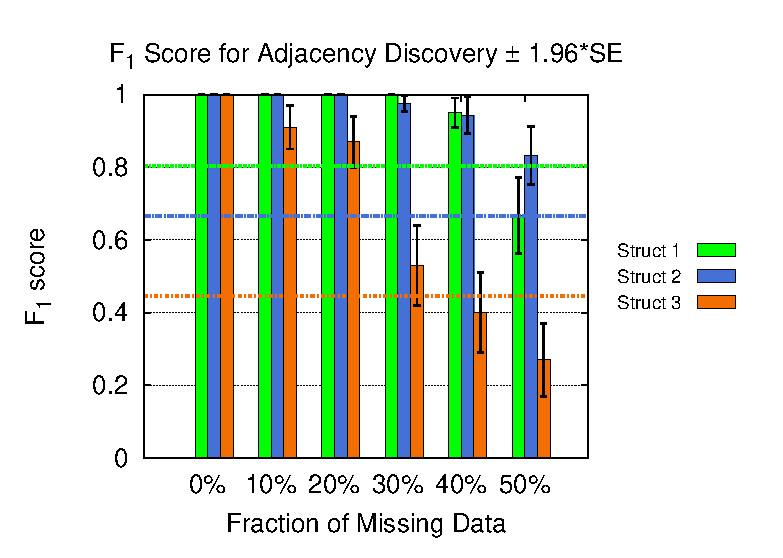
\includegraphics[width=1.1\linewidth]{figures/F1A_single_missing.eps} &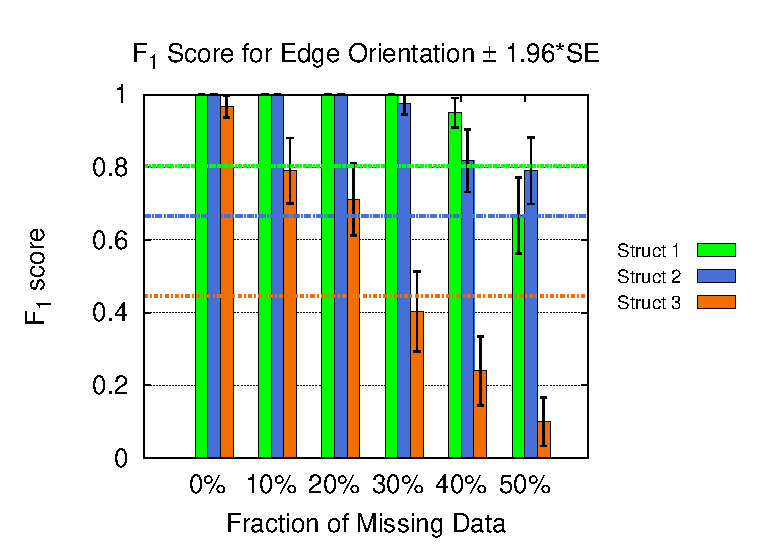
\includegraphics[width=1.1\linewidth]{figures/F1O_single_missing.eps}\\
					\end{tabular}
				\end{center}
				\vspace{-1em}
				\caption{Results of learning with missing data. Left: Comparison of $F_1$ scores for adjacency discovery. Horizontal lines are baseline $F_1$ scores computed for fully connected Bayesian networks. Right: Comparison of $F_1$ scores for edge orientation. }
				\label{fig:f1-missing} 
			\end{figure}

			\begin{figure}[ht]
						\begin{center}
							\centering
							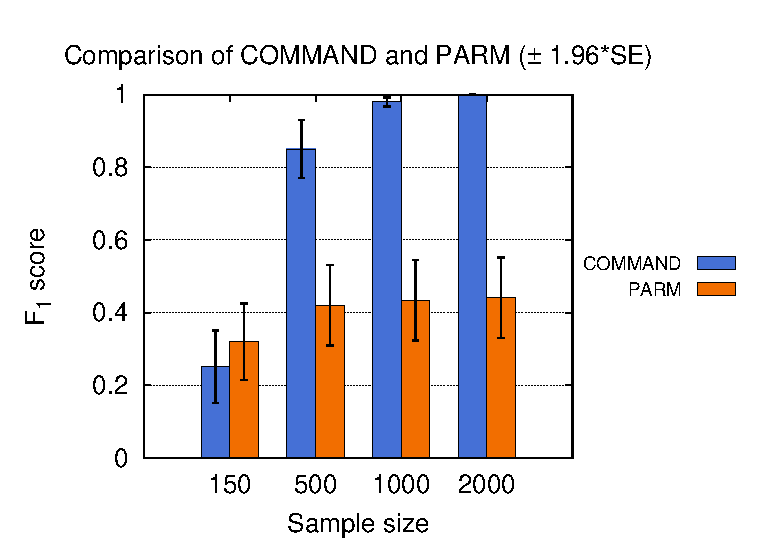
\includegraphics[width=0.55\linewidth]{figures/F1_parm.eps}
						\end{center}
						\vspace{-1em}
						\caption{Comparison of COMMAND and PARM for discovering prerequisite relationships in Structure 3. %The cutoff values used for PARM experiments are: $ minsup=0.125$, $minconf=0.76$, $minprob=0.9$.
						}
						\label{fig:f1-parm}
						\vspace{-1em} 
					\end{figure} 				
	\subsubsection{Comparison With Prior Work}
	The Probabilistic Association Rules Mining (PARM) is a recent algorithm for discovering the prerequisite relationships between skills~\cite{chen2015discovering}.
	In this approach, a prerequisite relationship $S_1\rightarrow S_2$ is considered to exist if
	$P(S_1=1,S_2=1) \ge minsup \wedge P(S_1=1|S_2=1)\ge minconf) \ge minprob$ and $P(P(S_1=0,S_2=0) \ge minsup \wedge P(S_2=0|S_1=0)\ge minconf) \ge minprob$, 
	where $minsup$, $minconf$ and $minprob$ are pre-specified constants between 0 and 1.

	
	We simulate data from Structure 3 from Figure~\ref{fig:syn-nets}(c) (with single-skilled items), which has 21 pair-wise prerequisite relationships.
	We derive pair-wise prerequisite relationships from this network  and see how the two approaches discover these relationships.
	When experimenting with PARM, we use $ minsup=0.125$, $minconf=0.76$, $minprob=0.9$, because they were suggested by the authors~\cite{chen2015discovering}.
	%\footnote{In PARM, a prerequisite relationship $S_1\rightarrow S_2$ is discovered if $P\left(P(S_1=1,S2=1) \ge minsup \wedge P(S_1=1|S_2=1)\ge ninconf\right) \ge minprob$ and $P(P(S_1=0,S_2=0) \ge minsup \wedge P(S_2=0|S_1=0)\ge minconf) \ge minprob$.} 
	%These values have been used in the simulation experiments in 
	
	%We compare two approaches using 
	%$F_1=\frac{2*TPR*TDR}{TPR+TDR}$, where $TPR=\frac{\text{\# of correct relationships learned}}{\text{\# of relationships in true model}}$
	%and $TDR=\frac{\text{\# of correct relationships learned}}{\text{\# of relationships in learned model}}$.
	
	PARM is limited to discovering pair-wise prerequisite relationships (instead of constructing the full structure).
	To make a fair comparison,  we evaluate how accurately COMMAND and PARM  discover relationship pairs.
	For this, we use the F1 metric in Table~\ref{tbl:ar}, but we count pairs of  \textit{related skills} instead of adjacencies.
	Two skills are related if one is a descendant of the other one.
	Figure~\ref{fig:f1-parm} shows that COMMAND  outperforms PARM, and the difference becomes significant for sample size $n\ge 500$.
	The low $F_1$ score of by PARM is %caused by low $TPR$, i.e., 
	%PARM 
	because it fails to discover many prerequisite relationships (data not shown), and because  PARM does not respect transitivity.
	For example, PARM may reject $S_1\rightarrow S_3$ even it has discovered $S_1\rightarrow S_2$ and $S_2\rightarrow S_3$.
	We speculate that selecting a different set of cutoff values for PARM may improve the results.
	However, determining these thresholds is not trivial and may require experts' intervention. By contrast, COMMAND does not require tuning. % of many parameters.
	%Further, the low $TPR$ is partially due to that PARM does not respect transitivity.
	%That is, given the cutoff values, PARM may reject $S_1\rightarrow S_3$ even it has discovered $S_1\rightarrow S_2$ and $S_2\rightarrow S_3$.
	%This seems quite 
	%Another problem of PARM is that it does not respect transitivity. 
	%That is, PARM may not identify $S_1\rightarrow S_3$ even when it has discovered $S_1\rightarrow S_2$ and $S_2\rightarrow S_3$.
	%This partially explains the low $TPR$.	 
	
			
			
		
					
	\subsection{Real Student Performance Data}
	\label{sec:real}
	We now evaluate COMMAND using two real-world data sets.	
	
	\subsubsection{English Data Set}
	The Examination for the Certification of Proficiency in English (ECPE) dataset describes 2922 examines in their understanding of English language grammar \cite{templin2014hierarchical}.
	%was collected from a test by the English language Institute... of the University of Michigan to examine individual cognitive skills required for 
	The dataset includes student performance in 28 items on 3 skills ($S_1$: morphosyntactic rules, $S_2$: cohesive rules,
	and $S_3$:lexical rules). Each item requires either one or two of the three skills.
	
				\begin{figure}[!th]
					\begin{center}
						\centering
						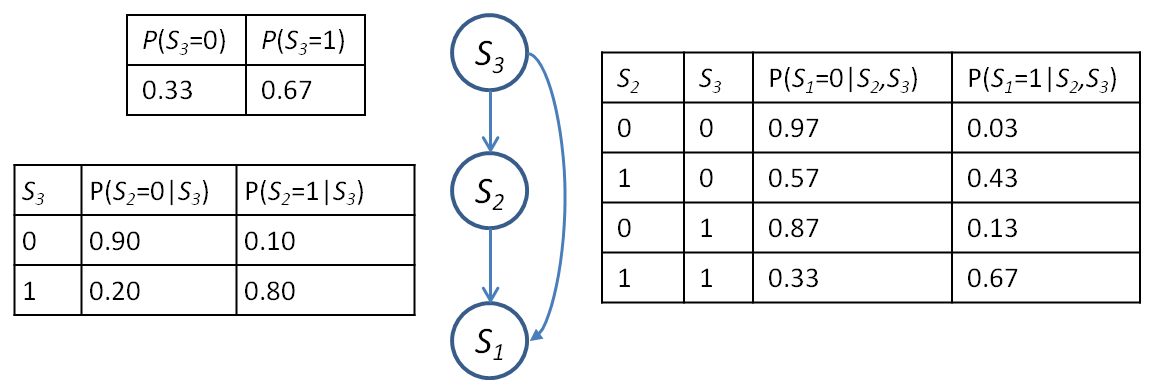
\includegraphics[width=0.95\linewidth]{figures/ecpe_results.png}
					\end{center}
					\vspace{-1em}
					\caption{%$S_1$: Morphosyntactic rules; $S_2$: Cohesive rules; $S_3$: Lexical rules. 
						The estimated DAG and CPTs of the ECPE data set.}
					\label{fig:ecpe-result} 
					%\vspace{-0.5em}
				\end{figure}
					 				
	Figure~\ref{fig:ecpe-result} shows the prerequisite structure discovered with COMMAND. %The estimated conditional probability tables (CPT) are showed correspondingly.
	It hypothesizes that lexical rules is a prerequisite of cohesive rules and morphosyntactic rules; 
	cohesive rules is a necessary skill for learning morphosyntactic rules. 
	The pair-wise prerequisite relationships totally agrees with the findings in \cite{templin2014hierarchical} and that by the PARM method in \cite{chen2015discovering}.
	%Note that PARM discovered the three pairwise prerequisite relationships but COMMAND output a full structure.
	Our model infers a complete DAG, suggesting that there are no conditional independencies among the three skills.
	This is an interesting insight that previous approaches cannot provide.   
	Further, COMMAND also outputs the conditional probabilities associated with each skill and its direct prerequisite.
%	which provides insights into how prerequisites impact the post-requisite probabilistically. 
	We clearly see that the probability of student mastering a skill increases when the student has acquired more prerequisites of the skill.
	
	
	\subsubsection{Math Data Set}
	We now evaluate COMMAND using data collected from a commercial non-adaptive tutoring system.
	The textbook items are classified in chapters, sections, and objectives.
	We only use  student performance data from tests in Chapter 2 and  3.
	That is, students are tested on the items after they have been taught all relevant skills.
	
	\paragraph{$Q$-matrix and preprocessing}
	\label{sec:preprocessing}
	We define skills as book sections.
	We use a $Q$-matrix that assigns each exercise to a skill solely as the book section in which the item appears.\footnote{Here we assume the items are single-skilled despite that they might be multi-skilled.}
	For each chapter, we process the data to find a subset of items and students that do not have missing values.
	That is, the datasets we use in COMMAND have students responding to \textit{all} of the  items.
	
	After filtering, two data sets, \texttt{Math-chap2} and \texttt{Math-chap3}, were obtained for Chapter 2 and 3 respectively. 
	In \texttt{Math-chap2}, six skills are included and each skill is tested on three to eight items, for a total of 30  items.
	In \texttt{Math-chap3}, seven skills are included and each skill has three to seven items, for a total of 33 items.
	\texttt{Math-chap2} includes student test results for 1720 students, 
	while the \texttt{Math-chap3} has test results for 1245 students.
	%Our synthetic data experiments suggest that a large number of training data improves the learning quality of the prerequisite structure.
	%For this reason, we use the larger \texttt{traditional} dataset to build the prerequisite model.
	For simplicity we use binary variables to encode  performance data and skill variables.
	%This simplification is not necessary,  as COMMAND is able to use  discrete variables with arbitrary number of states.
	
	\paragraph{Prerequisite Structure Discovery}
	\label{sec:prerequisite_results}
	
%			\begin{figure*}[!th]
%				\begin{center}
%					\centering
%					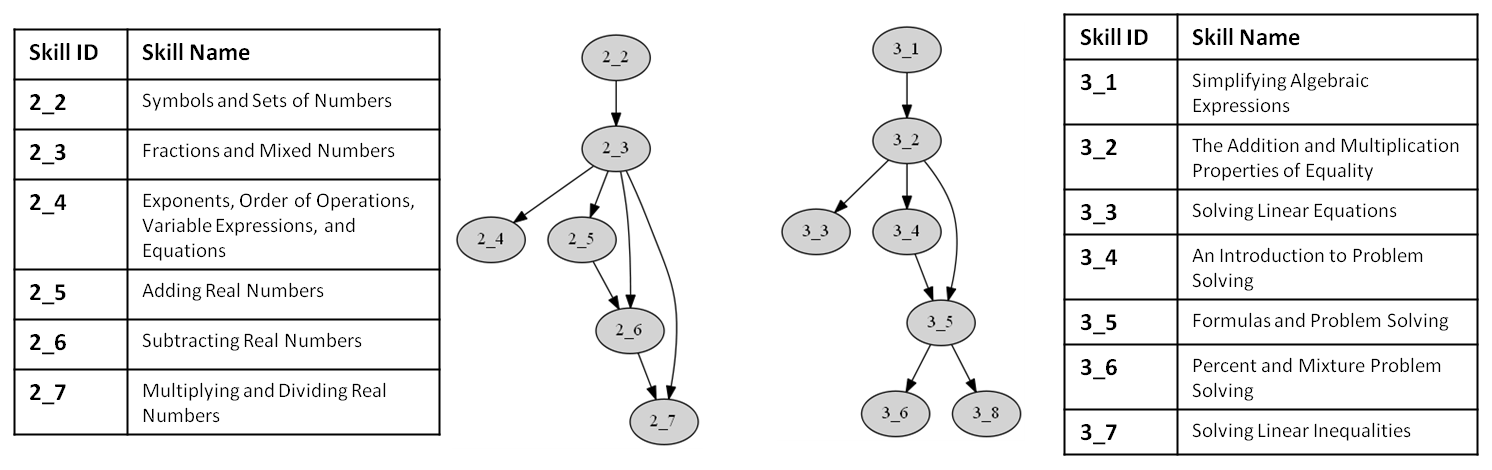
\includegraphics[width=1.0\linewidth]{figures/hed_structures.png}
%				\end{center}
%				\caption{Prerequisite structures constructed by COMMAND.}
%				\label{fig:hed-structures} 
%			\end{figure*}

	\begin{figure}[!ht]
		\centering
		\begin{subfigure}[b]{0.9\linewidth}
			\centering
			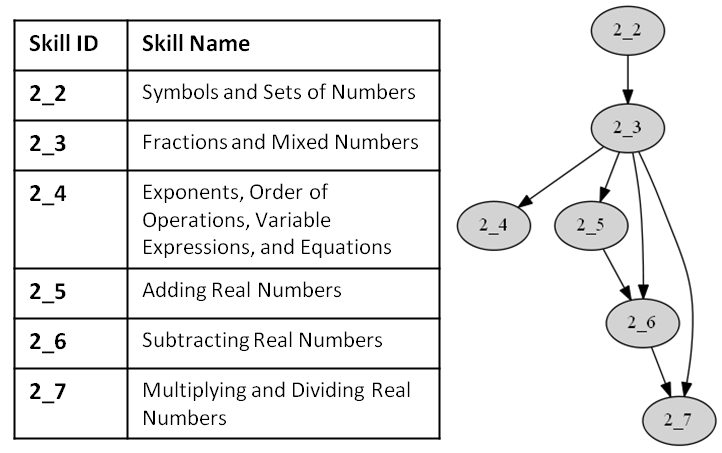
\includegraphics[width=0.9\linewidth]{figures/hed_chap2_structure_prob2.png}
			\caption{Prerequisite structure learned for \texttt{Math-chap2}.}
			\label{fig:hed_chap2_structure}
		\end{subfigure}\\
		\begin{subfigure}[b]{0.9\linewidth}
			\centering
			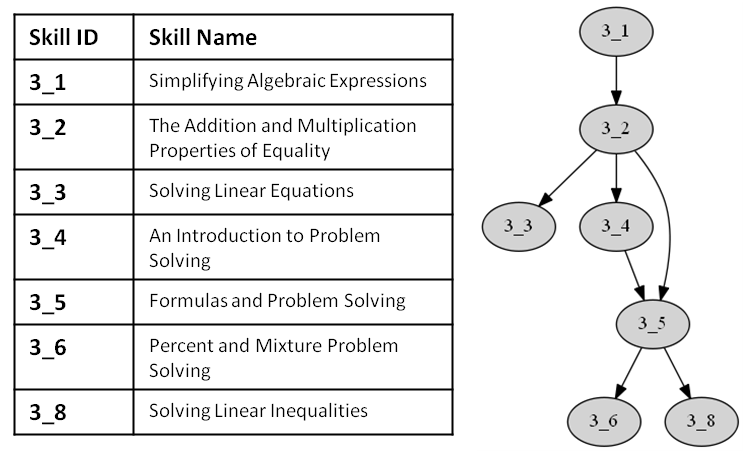
\includegraphics[width=0.9\linewidth]{figures/hed_chap3_structure_prob2.png}
			\caption{Prerequisite structure learned for \texttt{Math-chap3}.}
			\label{fig:hed_chap3_structure}
		\end{subfigure}%
		\caption{Prerequisite structures constructed by COMMAND for \texttt{Math} data sets.}
		\label{fig:hed-structures}
		%\vspace{-1em} 
	\end{figure}			
	
	The Bayesian networks generated with the COMMAND algorithm are illustrated in Figure~\ref{fig:hed-structures}.
	%Figure~\ref{fig:qmatrix} represents a disconnected model generated by simply converting the input $Q$-matrix into a Bayesian network;
	%this corresponds to the output of the initialization step of Algorithm~\ref{alg:remind}.
	%Figures~\ref{fig:constraint} and~\ref{fig:noconstraint} represent the prerequisite structures discovered by using domain knowledge or not.
	%In the fully data-driven model, we draw with red the edges that contradict our text book ordering heuristic.
	%Note that some edges are undirected indicating these directionalities of these edges can not determined given the observational data.
	%Our observation is that the structures learned are not random, sections (skills) in the same chapter tend to form clusters, 
	%even in the structure learned without the ordering constraint.
	Our observation is that the topological order of the sections in both structures are fully consistent with the book ordering heuristic.
	This shows an agreement between our fully data-driven method and human experts.
	We also ran PARM approach to learn pair-wise prerequisite relationships from these data sets. Given $minsup=0.125$, $minconf=0.76$ and $minprob=0.9$,
	$2\_5\rightarrow 2\_6$, $2\_5\rightarrow 2\_7$ and $2\_6\rightarrow 2\_7$ are discovered for \texttt{Math-chap2},
	$3\_1\rightarrow 3\_3$ and $3\_2\rightarrow 3\_3$ are discovered for \texttt{Math-chap3}.
	These relationships are small subset of the set of relationships discovered by COMMAND. 
	%The inferred prerequisite structures are intuitively plausible, 
	%as the topological order of the sections are consistent with the book structure, which reflects subject matter experts's belief on the prerequisite relationships 
	%between the sections of each book chapter. 

%	Our approach also outputs the conditional probabilities associated with each skill and its direct prerequisites.
%	Figure~\ref{fig:chap123noorderCPT} plots the conditional distribution table for each skill.
%	Each sub-figure plots the conditional probability of student achieving the mastery of a skill against the mastery status of the skill's direct prerequisites. 
%	More specifically, X-axis specifies all possible mastery statuses of a skill's direct prerequisite, 
%	Y-axis is the probability of student achieving the mastery of the skill given the corresponding mastery status of its direct prerequisites.
%	We can see a trend in all plots that the probability of student mastering a skill increases monotonically when the student has acquired more prerequisites of the skill.
%	This is consistent with our intuition that mastering a skill's prerequisites will help student master the skill.
%	We also observed a small contradiction in the case of skill 3-2, which exemplifies the limitation of fully data-driven methods. 
	%\hl{Please describe this figure with much more detail than this.  This currently does not have enough explanation to be understandable}
	
	\paragraph{Predictive Performance}
	\label{sec:predictive_performance}
	COMMAND outputs a  Bayesian network model that can be used for inference and predictive modeling.
	For example, given a student's response to a set of items, we can infer the student's knowledge status of a skill.
	We could use COMMAND to identify students that may need  remediation because they lack some background.
	%We now evaluate  REMIND using data  that has already been collected (\textit{post-hoc} analysis). %an evaluation of the REMIND algorithm using  . 
	We evaluate the accuracy of the predicted student performance  on an item, when we observe the student response on the other items.
	%student's knowledge about a skill given his/her performance on any of the test items. 
	%Since student's knowledge about a skill is not directly observed, 
	%we are unable to assess the predictive performance of these models involved in this task.
	%However, we have direct observations on students' performance on test items. 
	%For this, we evaluate  predicting student performance
%	on a test item given response on other items.
	More precisely, we compute the posterior probability of a student's response to an item $I_i$ given his performance on all other items 
	$\mathbf{I}_{-i}=\mathbf{I}\setminus\{I_i\}$, by marginalizing over the set of latent variables $\mathbf{S}$:
\[
		P(I_i|\mathbf{I}_{-i}=\mathbf{i}_{-i}) =\sum_{\mathbf{S}}P(I_i, \mathbf{S}|\mathbf{I}_{-i}=\mathbf{i}_{-i}).
\]
	
	This probability can be computed efficiently using the Junction tree algorithm~\cite{koller2009probabilistic}. 
	We then do binary classification based on the posterior probability to determine if the student is likely to answer correct.
	We compare the Bayesian network models generated from COMMAND with five baseline predictors:
	\begin{itemize}[topsep=2pt,parsep=0pt,partopsep=0pt]
		\item  A \emph{majority} classifier which always classifies  an instance to the majority class.
		For example, if majority of the students get an item wrong, other students would likely get it wrong.
		\item  A Bayesian network model in which the skill variables are \emph{disconnected}. 
		%This corresponds to using the $Q$-matrix  Bayesian network of Figure~\ref{fig:qmatrix}.
		This model assumes that the skill variables are marginally independent of each other. Most existing knowledge tracing approaches make this assumption.
		\item A Bayesian network model in which the skill variables are connected in a \emph{chain} structure, i.e., 2-2$\rightarrow$2-3$\rightarrow$2-4$\rightarrow\dots$
		This assumes that a section (skill) only depends on the previous section.
		In other words, a first-order Markov chain dependency structure.
		\item A Bayesian network model constructed using the pairwise relationships output from \emph{PARM}. 
		That is, we create an edge $S_i\rightarrow S_j$ if PARM says $S_i$ is the prerequisite of $S_j$.
		\item A \emph{fully connected} Bayesian network where skill variables are fully connected with each other.
		This model assumes no conditional independence between skill variables and can encode any joint distribution over the skill variables.
		However, it has exponential number of free parameters and thus can easily overfit the data.
	\end{itemize}
	\begin{figure}[!ht]
		\centering
		\begin{subfigure}[b]{0.48\linewidth}
			\centering
			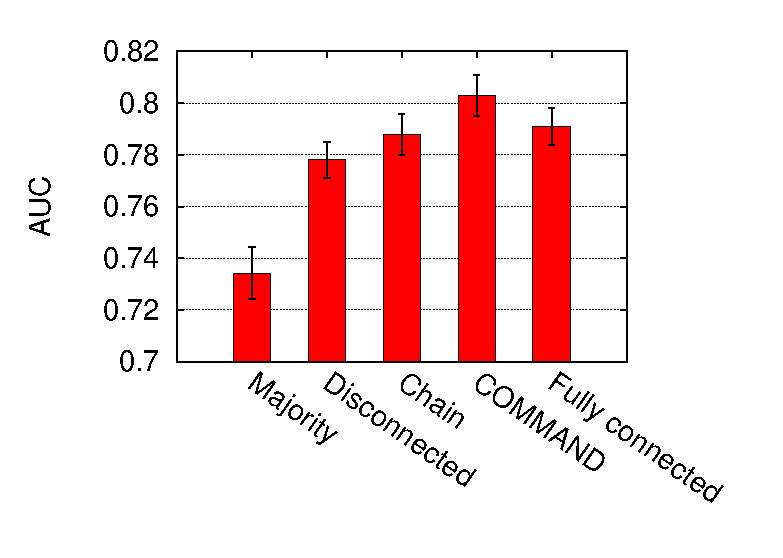
\includegraphics[width=1.1\linewidth]{figures/hed_chap2_30_auc.eps}
			%\vspace{-1em}
			\caption{\texttt{Math-chap2} AUC results. }
			\label{fig:auc-chap2}
		\end{subfigure}
		\begin{subfigure}[b]{0.48\linewidth}
			\centering
			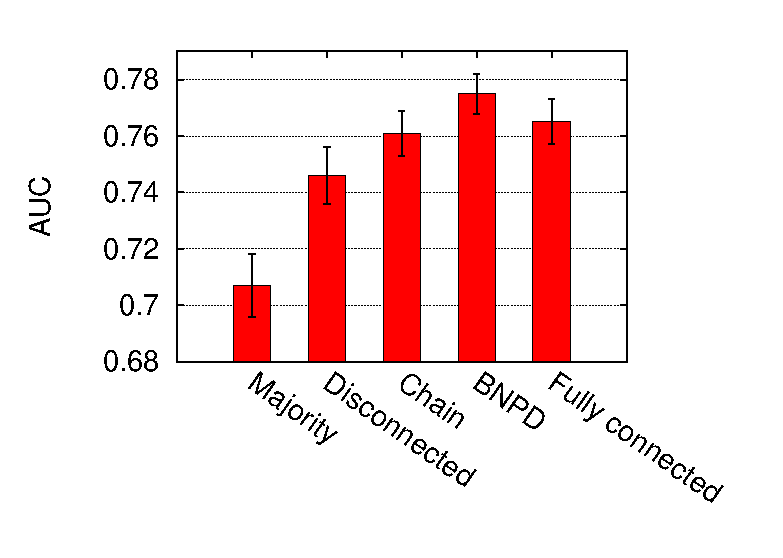
\includegraphics[width=1.1\linewidth]{figures/hed_chap3_33_auc.eps}
			%\vspace{-1em}
			\caption{\texttt{Math-chap3} AUC results.}
			\label{fig:auc-chap3}
		\end{subfigure}%
		%\vspace{-0.5em}
		\caption{Ten fold cross-validation results of evaluating the predictions of student performance.} %\hl{why does the y-axis start at 0.68? consider 0.5}
		\label{fig:aucs}
		%\vspace{-1em}
	\end{figure} 	
	
	The parameters of these baseline Bayesian network predictors are estimated from the data using parametric EM.
	The model predictions were evaluated using the \textit{Area Under the Curve} (AUC) of the Receiver Operating Characteristic (ROC) curve metric 
	calculated from 10-fold cross-validation.
	Results are presented in Figure~\ref{fig:aucs}. 
	The error bars show the $95\%$ confidence intervals calculated from the cross-validation.
	On both \texttt{Math-chap2} and \texttt{Math-chap3} data sets, the COMMAND models outperform the other five models.
	The \emph{fully connected} models are the second best performing models.
	On \texttt{Math-chap2}, COMMAND model has an AUC of $0.803\pm0.008$ and the \emph{fully-connected} model has an AUC of $0.791\pm0.007$ (Figure~\ref{fig:auc-chap2}).
	A paired $t$-test reveals that the AUC difference of two models are statistically significant with a $p$-value of $0.0022$.
	On \texttt{Math-chap3}, COMMAND model has an AUC of $0.775\pm0.007$ and the \emph{fully-connected} model has an AUC of $0.765\pm0.008$ (Figure~\ref{fig:auc-chap3}).
	The AUC difference of two models are also statistically significant with a $p$-value of $0.01$.
	The \emph{fully connected} models are outperformed by the much simpler prerequisite models, suggesting overfitting.
	
	
	%(Figure~\ref{fig:auc-chap2}), respectively. % and correspond to and no constraints, respectively.
	%these models are: $0.691\pm0.011$ (\emph{majority}), $0.761\pm0.007$ (\emph{disconnected}), $0.796\pm0.006$ (\emph{chain}),  $0.804\pm0.007$ (\emph{prerequisite model with order constraint}), $0.807\pm0.006$ (\emph{prerequisite model without order constraint}), $0.794\pm0.007$ (\emph{fully connected}).
	%The comparison of the Area Under Curve (AUC) \todo{Area of what curve? ;-)} for these classifiers is presented in Figure~\ref{fig:auc-cv}.
	%These two REMIND models outperform the other four models.
	%\hl{How much is the AUC, though? Explain the graph with words here}
	%We note that the \emph{fully connected} model was outperformed by the two prerequisite models and the \emph{chain} model, suggesting  overfitting.% might have happened. 
	
	
	\section{Conclusion and Discussion \label{sec:conclusion}}
	%Discovering prerequisite structures of skills from data is challenging since skills are latent variables in the data.
	Prerequisite graphs have been shown~\cite{botelho2015prediction,kaser2014beyond} to improve student models.
	However, discovering the prerequisites between skills requires significant effort from subject matter experts.
	%We demonstrate with fully data-driven prerequisite structures.
	The main contribution of our work is a novel algorithm that simultaneously infers a prerequisite graph and a student model from data with less human intervention.
	%We converted the prerequisite discovery problem to a problem of Bayesian network structure learning with latent variables.
	%We introduced the Structural EM
	%We demonstrate our approach using both synthetic and real-world data.
	
    We  extend  on prior work in significant ways.
	We optimize the full structure of skills that captures the conditional independence between skills, instead of only estimating the pairwise relationships.
	Our experiments suggests that this results in better accuracy.
	Moreover, we argue that our strategy is  easier to use %more the quality of the discovered prerequisite structures discovered.
	%We believe COMMAND is easier to use
        because  it does not require  manual tuning of  parameters.
	Other methods~\cite{brunskill2010estimating} require the  \emph{guess} and \emph{slip} probabilities to be  provided as input,
	or alternatively~\cite{chen2015discovering},  thresholds to determine the existence of a prerequisite relationship.
	Determining these values requires experts' intervention. 
	COMMAND does not require such tuning.
	%In contrast, the only required input to our algorithm is the observed student performance. and the $Q$-matrix.
	
	We analyze how missing values, noise and dataset size can affect the performance of COMMAND.
	Further research could explore additional datasets and baselines.
	A secondary contribution of our work is that we develop a methodology to evaluate  prerequisite structures on real student data.
	We believe that we are the first to compare prerequisite discovery strategies by how well they can be used to predict student performance.
	Therefore, we validate COMMAND not only with synthetic data, but with two real-world datasets.
	Our results suggest that COMMAND improves on the state of the art  because it significantly improves on a recently published technique.
	
	 % it under different conditions, such as  missing values and noise.
	%Overall, we believe that our work is useful to improve student modeling.
	%Future work can investigate how to use COMMAND to create remedial interventions.
	
	Learning a prerequisite graph is not merely discovering a Bayesian network--- 
	   equivalent Bayesian network structures  in fact represent different prerequisite structures.
	%Studying prerequisite structure discovery in the context of Bayesian network structure learning is not new \cite{scheines2014discovering}.
	%However, the approach in \cite{scheines2014discovering} does not discriminate between equivalent Bayesian network structures which represent different prerequisite structures.
       We believe we are the first to address this problem.
       We use domain knowledge to refine the prerequisite models output using a theoretically motivated method.
%	In future, it would be wiser to refine the model within the Structural EM learning. 
%	For example, in Structural EM search, we can use a scoring function with an additional term that penalizes the structures that violate the domain knowledge. 
%	In such way, learning may be more accurate.
	%Overall, we believe that our work improves the state-of-the-art of student modeling.
	

	

	
	%Our approach differs from prior work in several ways.
	%First, most of existing approaches focus on estimating the pairwise prerequisite relationships \cite{brunskill2010estimating,chen2015discovering}.
	%By contrast, we try to optimize the full structure of the model by converting the problem to a problem of Bayesian network structure learning with latent variables.
	%Studying prerequisite structure discovery in the context of Bayesian network structure learning has been explored By Scheines and his colleagues in \cite{scheines2014discovering}.
	%However, due to the Markov equivalence between Bayesian network structures, the model output from their approach is inaccurate and can represent different prerequisite structures.
	%Our approach discriminates between the equivalent Bayesian network using constraints derived from the domain knowledge of prerequisite relationship. 
	
	%We believe we are the first ones to propose an algorithm of learning the prerequisite dependencies from data and use it for student modeling. 
%	Our work builds on prior work that discovers prerequisite from data \cite{desmarais2006learned,vuong2010method, brunskill2010estimating,scheines2014discovering,chen2015discovering,piech2015deep}.
%	However, these approaches do not attempt to validate the prerequisite discovered using real student performance data.
%	Our approach differs from prior work in several ways.
%	The approaches discover the relationship of items without using latent variables.
%	This is, the prerequisites do not use skill mappings, and only find dependencies between items~\cite{desmarais2006learned,vuong2010method,piech2015deep}.
%	%i.e., the item-level prerequisite relationships, while we try to discover the prerequisite relationships between hidden skills.
%	For the approaches that can account for latent variables~\cite{brunskill2010estimating,chen2015discovering}, they focus on estimating the pairwise prerequisite relationships.
%	By contrast, we try to optimize the full structure of the model.
	
	%A contribution of our work is introducing the Structural EM algorithm to the educational community.
%	Our approach has many advantages over prior work. First, it does not require tuning of many parameters.
%	For example, prior work~\cite{brunskill2010estimating} assumes domain parameters called \emph{guess probability} and \emph{slip probability}
%	%\footnote{The \emph{guess probability} is the probability of answering the correctly given the student does not know the skill; the \emph{slip probability} is the probability of answering incorrectly given the student knows the skill} 
%	are provided for each pair of item and skill while COMMAND learns these parameters automatically.
%	Similarly, more recent approaches~\cite{chen2015discovering} require manually specified thresholds to determine the existence of a prerequisite relationship.
%	The determination of these thresholds requires experts' intervention. 
%	By contrast, the only required input of our algorithm is the observed student performance.
%	Further, these methods discover pair-wise relationships while COMMAND tries to optimize the full structure of the model.	
	

	%\hl{Two parts: Prerequisite discovery and student modeling with multiple kcs}
	%\hl{For prereq work: Cite Ilya's work, French lab, Thorsten's work, may be Deep KT work}
	%\hl{Have a comparative table of prereq work}
	%\hl{For student modeling with multiple KCs cite LR-DBN work by YanBo, Topical HMM \&FAST work by Jose, conjunctive kt by Ken Koedinger}
	
%	Although in some educational paradigms~\cite{koedinger2010knowledge} students are not supposed to move to subsequent lessons until they have mastered all of the prerequisites, these is not always attainable in practice.
%	We propose and evaluate the REMIND pipeline, a simple but effective novel algorithm that detects when a student needs remediation.
%	
%	A limitation of our study is that we only evaluated REMIND using simulations and posthoc analyses.
%	Future work may evaluate the REMIND algorithm in a randomized control trial.
%	Further, we evaluated our models using traditional statistical metrics, 
%	but recent work suggest that tailored evaluation metrics for tutoring system may be superior \cite{leopard_edm}.
%	Thus, another piece of future work is to evaluate REMIND using these evaluation metrics.
%	
%	The main contributions of our work are:
%	a novel data-driven algorithm that allows domain knowledge for designing remediation triggers;
%	a novel methodology to evaluate prerequisite graphs using student data;
%	and suggesting the Structural EM algorithm for educational applications.
%	
%	The advantage of REMIND are both qualitative and quantitative.
%	Qualitatively, REMIND allows us to understand the organization of the skills in the curriculum as it builds a prerequisite network of the skills in a $Q$-matrix.
%	When used in a learning model, REMIND builds a hypothesis of how practice affects the knowledge of the student.
%	Sometimes the practice may affect the skill directly, but sometimes it may affect a prerequisite.
%	Future work may validate these hypothesis in a controlled experiment.
%	Additionally, our quantitative results suggest that REMIND can be used to improved student modeling.
%	Overall, we believe that REMIND is promising technology to detect when a student needs help.
	
% REFERENCES FORMAT
% References must be the same font size as other body text.
\bibliographystyle{SIGCHI-Reference-Format}
{\small
	\bibliography{references}
}	

\end{document}
